\chapter{Inverse Synthesis Experiment}
\label{chapter:inverse_synth_experiment}

This chapter presents an inverse synthesis experiment that was conducted to compare recent approaches that have been used in previous work. The methodology used for this experiment was modelled after Yee-King et al.'s study on deep learning for automatic synthesizer programming \cite{yee2018automatic}, but with a simplified synthesizer configuration and a unique set of estimators. In total eleven different methods for inverse synthesis were compared, including eight deep learning models based on previous work \cite{barkan2019inversynth, yee2018automatic}, two versions of a genetic algorithm \cite{horner1993machine, tatar2016automatic}, and a novel hybrid approach that combines deep learning and genetic algorithms. A VST software emulation of the Yamaha DX7 FM synthesizer called \textit{Dexed} was used with a restricted subset of the parameters. While Dexed has been used in previous work for inverse synthesis \cite{yee2018automatic, luke2019stochastic, le2021improving, masudo2021quality}, each work has used a unique subset of parameters and sounds for their experiments. The difficulty of the problem varies considerably depending on the number of parameters selected. In this experiment I propose a minimal subset of seven parameters to reduce the complexity of the problem and to provide a benchmark for evaluation.

The specific research questions that this experiment seeks to answer are:
\begin{itemize}
    \item \textbf{RQ1}: How do deep learning approaches compare to genetic algorithms for FM inverse synthesis?
    \begin{itemize}
    	\item Are the GAs able to produce competitive results when constrained to a limited number of generations to improve efficiency?
    	\item Can GAs be combined with deep learning approaches to improve both efficiency and accuracy?
    \end{itemize}
    \item \textbf{RQ2}: What deep learning approaches are best for FM inverse synthesis?
    \begin{itemize}
    	\item How do RNNs compare to CNNs?
    	\item How does the audio representation affect the deep learning models?
    	\item Do higher resolution Mel-spectrograms afford a benefit over MFCCs?
    \end{itemize}
    \item \textbf{RQ3}: Are certain synthesis parameters more easily learned? How does the ability to predict parameters correlate with audio results?
\end{itemize}

% Add a bit of a summary on the results here
%Results show that 

% Add in some specific research questions?
% RQ1: How do deep learning methods compare genetic algorithms for FM inverse synthesis?
% RQ2: How do the RNNs compare to the CNNs - and do higher resolution Mel-spectrograms allow the CNNs to learn more accurately compared to the RNNs using MFCCs?
% RQ3: Are the genetic algorithms able to produce competitive results when constrained to a limited number of trials and population size?
% RQ4: Are certain parameters more easily learned? Are parameters that control temporal aspects vs. frequency components more easy to estimate?


The following section describes in more detail the methods used for this experiment including the precise configuration of the synthesizer, the dataset used for training, and the various techniques compared. Section \ref{sec:inverse-synth-eval} describes the methods used for evaluation and the results of this evaluation. Section \ref{sec:inverse-synth-discuss} presents a discussion of the results and some of the challenges associated with the inverse synthesis problem. In alignment with Vandewalle et al.'s criteria for reproducible research, implementation details, code, and datasets are all available on the \mintinline{python}{spiegelib} online documentation.\footnote{\url{https://spiegelib.github.io/spiegelib/examples/fm_sound_match.html}}

\section{Synthesizer Configuration}
The first step in the experiment was defining the synthesizer setup. The $Dexed$ VST instrument was selected for this experiment for a number of reasons: 1) it is an FM synthesizer that is modelled closely after the Yamaha DX7 synthesizer which is both widely used as well as notoriously difficult to program, 2) Dexed is open-source and free to use which makes it easy for the results to be reproduced, and 3) it has been used in a number of previous works on inverse synthesis \cite{yee2018automatic, luke2019stochastic, le2021improving, masudo2021quality}. An image of the $Dexed$ interface is shown in figure \ref{fig:dexed}. Dexed has 155 parameters that are available for external manipulation and for inverse synthesis. A subset of seven of these parameters were used in this experiment to turn $Dexed$ into a simple two-operator FM synthesizer. In this configuration the second operator modulates the frequency of the first operator. A block diagram showing the resulting synth configuration is shown in figure \ref{fig:two_op_fm_block}. The subset of seven parameters control the amplitude envelope and tuning of the modulating oscillator; this simple synthesizer can produce a wide range of timbres that evolve in various ways over time based on the amplitude envelope of the modulating oscillator. An overview of these seven parameters is given in table \ref{tbl:dexed-params}.

\begin{figure}[ht]
    \centering
    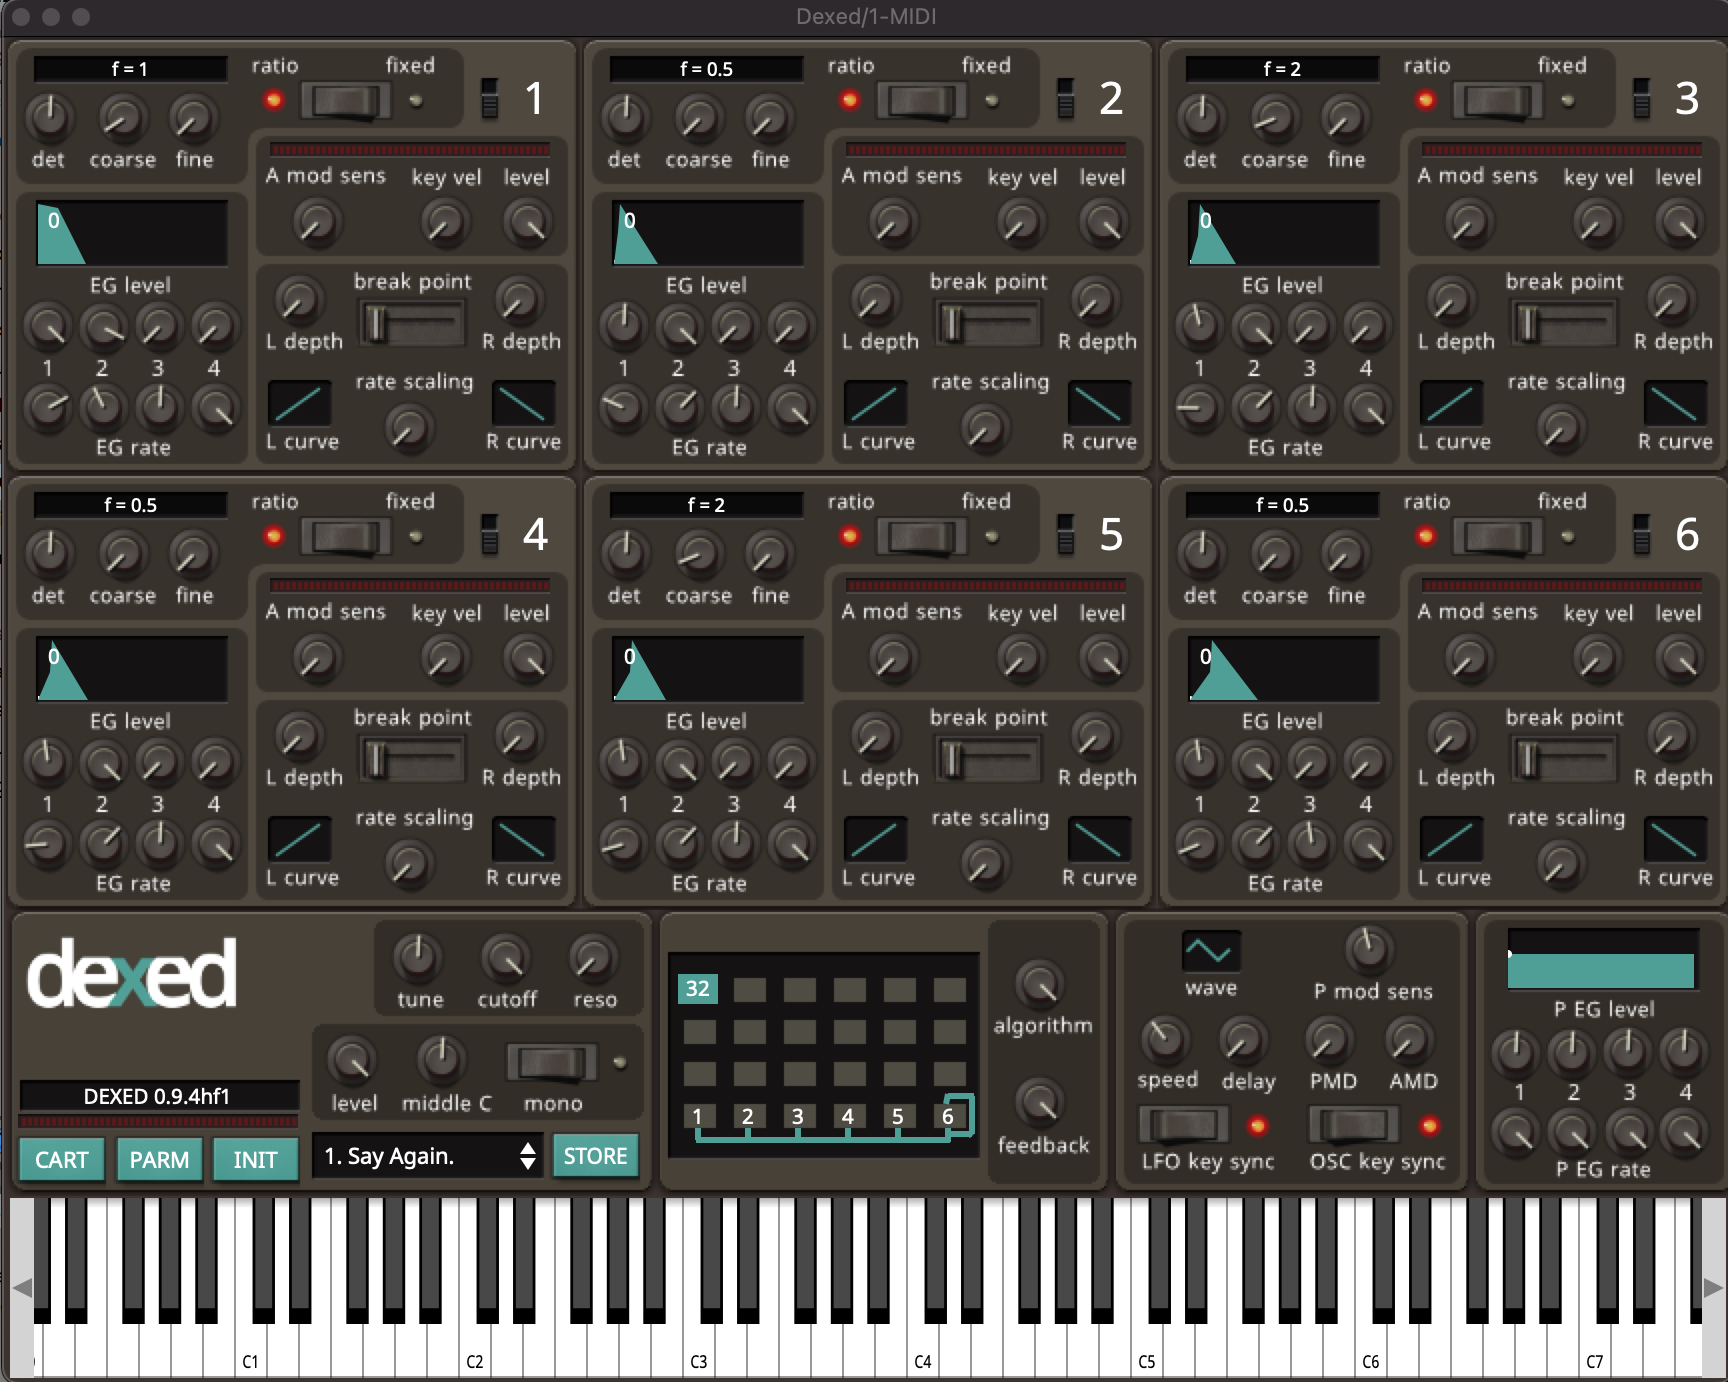
\includegraphics[width=0.6\textwidth]{figures/spiegelib/dexed.png}
    \caption{The Dexed synthesizer interface. Dexed is an open-source emulation of the Yamaha DX7 FM synthesizer and it was used in the experiments in this chapter/}
    \label{fig:dexed}
\end{figure}

\begin{figure}[ht]
    \centering
    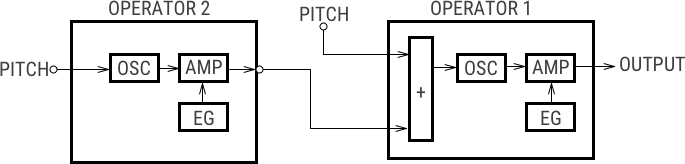
\includegraphics[width=0.9\textwidth]{figures/spiegelib/two_op_fm_block.png}
    \caption{Block diagram of a two operator FM synthesizer. Dexed has six independent operators that can be configured in various ways, however for the experiments conducted here only the first two operators were used and were setup in this configuration.}
    \label{fig:two_op_fm_block}
\end{figure}

\begin{table}[ht]
\centering
\caption{Synthesis parameters used in experiment}
\label{tbl:dexed-params}
%\def\arraystretch{1.5}%  1 is the default, change whatever you need
\begin{tabular}{l|l}
\toprule
Parameter     & Description                                                                                  \\
\midrule
OP2 EG RATE 1 & \multirow{3}{*}{\parbox{0.70\linewidth}{Controls the duration of stages 1-3 of the envelope generator applied the the amplitude of operator 2}} \\
OP2 EG RATE 2 \\
OP2 EG RATE 3 \\
\midrule
OP2 EG LEVEL 2 & \multirow{2}{*}{\parbox{0.6\linewidth}{Controls level of the envelope generator at stages 2 and 3, which is applied the amplitude of operator 2}} \\
OP2 EG LEVEL 3 \\
\midrule
OP2 F COARSE & \multirow{2}{*}{\parbox{0.6\linewidth}{Frequency of second operator in relation to the fundamental frequency of the MIDI pitch. Coarse tuning is an integer ratio from $\frac{1}{2}$ to 31. Fine tuning allows for smaller non-integer adjustments.}} \\[2.75ex]
OP2 F FINE \\[2.75ex]
\bottomrule                                                                                        
\end{tabular}
\end{table}
\vspace{1cm}

\subsection{Amplitude Envelope}
Each operator in $Dexed$ has a complex envelope generator (EG) that is used modulate the amplitude of that operator. The complex envelope generator has five independent stages that are controlled by a set of parameters that are used to adjust the length and amplitude of each stage. See figure \ref{fig:dx7_envelope} for a diagram of an EG. For this experiment, only the EG for the second operator was modifiable, the EG for the first operator was set to produce a fully open amplitude envelope. Five parameters for the second operator were modifiable: Rate $1-3$, and level 2 and 3. Level 4, the start of the envelope, was locked to zero, and level 1 was locked to one, the maximum value. This meant that the start of the envelope always consisted of an attack starting from zero and rising to one over a duration set by rate 1. The release portion of the envelope was not included during audio generation so rate 4 was negligible.

\subsection{Operator Tuning}
Two parameters controlling the tuning of the second operator were also modifiable: coarse tuning and fine tuning. The tuning is in relation to the fundamental frequency of the midi pitch and first operator. Integer ratios produce harmonic overtones and non-integer ratios produce more dissonant timbres.

\subsection{Other Parameters}
The remainder of the parameters were locked to values such that the first operator would create a static sine wave with no amplitude modulation for the entire duration of a MIDI note. All of the other operators, modulation, and effects processors in Dexed were turned off. This meant that all the variation in possible sounds in this synthesizer configuration are produced through varying frequency and amplitude of the second operator, which is modulating the first operator. The \mintinline{python}{SynthVST} class in spiegelib provides methods for overriding and freezing parameters as well as saving and loading parameter settings as JSON files. 

%
% Although each of the included parameters control the amplitude EG and pitch of the operator in distinct ways, there is redundancy in the parameter spaced, i.e. different parameter settings could lead to the same auditory result. This redundancy represents one of the complexities of synthesizer parameter spaces and challenges in automatic synthesizer programming. This experiment intentionally seeks to explore the affect this redundancy has on each techniques ability to effectively match. All parameters have a normalized range from $[0-1]$ and mapping from this normalized range is handled internally by the Dexed code. The remainder of the available parameters in $Dexed$ are locked at values to create a simple sine wave generator that is being frequency modulated by the second operator. [ADD A TABLE IN APPENDIX FOR ALL THE PARAMETER VALUES]. The \mintinline{python}{SynthVST} class in spiegelib provides methods for overriding and freezing parameters as well as saving and loading parameter settings as JSON files. 

\begin{figure}[ht]
    \centering
    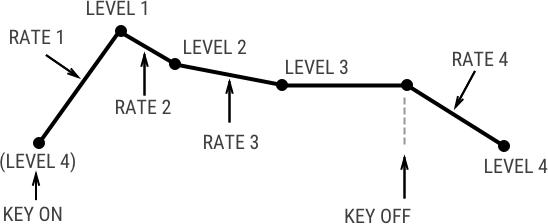
\includegraphics[width=0.75\textwidth]{figures/spiegelib/Yamaha DX7 Envelope.png}
    \caption{Diagram of an envelope generator in the Yamaha DX7 and Dexed. The envelope has five independent stages. During the first three stages the envelope moves linearly from level 4 to level 1, then to level 2, then to level 3. Each of these levels is controllable and the length of time taken to move to each level is also definable. This movement is triggered by a key-on event. Once the envelope has progressed to level 3 it stays at that level until a key-off event is received, at which point the envelope progresses back to level 4.}
    \label{fig:dx7_envelope}
\end{figure}


\section{Dataset Generation}
\label{sec:dataset-generation}

A dataset of synthesized audio paired with the parameters was required for training the deep learning models. Creating this dataset consisted of four steps: 1) sampling the parameter space, 2) playing a single note on Dexed with those parameters, 3) saving the audio and parameters, and 4) transforming the audio into a suitable audio representation. All audio was rendered by playing a single MIDI note on Dexed with a note value of 48 (C3 - $\approx 130.81$Hz) and length of one second. 80,000 examples were generated by uniformly sampling the seven parameters and rendering audio for one second. As mentioned previously, the release portion of the EG was left out, this is due to the render length and note length being the same.

The audio and parameter values were saved and the dataset was then split into a training and validation set with the training set containing 80\% of the samples. Once the audio dataset was created, audio representations were generated for each example.

\subsection{Audio Representations}
All the models received audio input that has been transformed into a more perceptually relevant representation. Two different representations were compared. Mel-frequency cepstral coefficients (MFCCs) have been used by Yee-King \textit{et al.} \cite{yee2011automatic, yee2018automatic} for automatic synthesizer programming and are included here as well. The second representation used in this experiment are log Mel-spectrograms. Barkan \textit{et al.} \cite{barkan2019inversynth} used a STFT representation in their experiments with CNNs, however Mel-spectrograms provide a more perceptually relevant frequency scaling and have been used in recent work in audio representations \cite{cramer:learnmore:icassp:19, hershey2017cnn}. 

The MFCCs were computed with 13-bands using a frame size of 2048 and a hop size of 1024, this resulted in 44 frames over the 1-second long input audio. To compute the Mel-spectrograms, a STFT was first computed using a frame-size of 2048 samples and a hop-size of 1024 samples. Each frame of the magnitude spectrogram was then converted to a power spectrum and projected onto a 64 component Mel-frequency scale. The resulting Mel-spectrogram was then scaled to a log-scale, an amplitude scaling more reflective of how the human auditory system perceives loudness. Equation \ref{ref:eq-log-scale} shows the calculation of the log-scaled Mel-spectrogram from a complex valued spectrogram, $\textbf{X}$, where $\textbf{M}$ is a matrix of weights to project each frame in the spectrogram onto 64 Mel-frequency bins.

\begin{align}\label{ref:eq-log-scale}
    \textbf{X}_{logmel} &= 10*log_{10}(|\textbf{X}|^2 \cdot \textbf{M})
\end{align}

Both audio representations were standardized to have zero mean and unit variance. An example of the resulting representations computed on a the same audio sample is shown in figure \ref{fig:mfcc-mel-representations}. Both the MFCC and Mel-spectrogram representations show an envelope in the signal starting at the beginning of the sound and lasting until about 0.45 seconds. The Mel-spectrogram gives a much higher resolution perspective of the frequencies present in the signal, whereas the MFCC only captures the overall shape of the spectral envelope and provides a much more compact representation. Pitch information is lost with MFCCs, which was identified by Masuda \textit{et al.} as an issue for synthesizer sound matching applications \cite{masudo2021quality}. However, Yee-King \textit{et al.} has achieved good results using MFCCs, so they are were included for comparison to the higher-resolution Mel-spectrograms.

\begin{figure}[ht]
    \centering
    \begin{subfigure}[b]{0.45\textwidth}
        \centering
        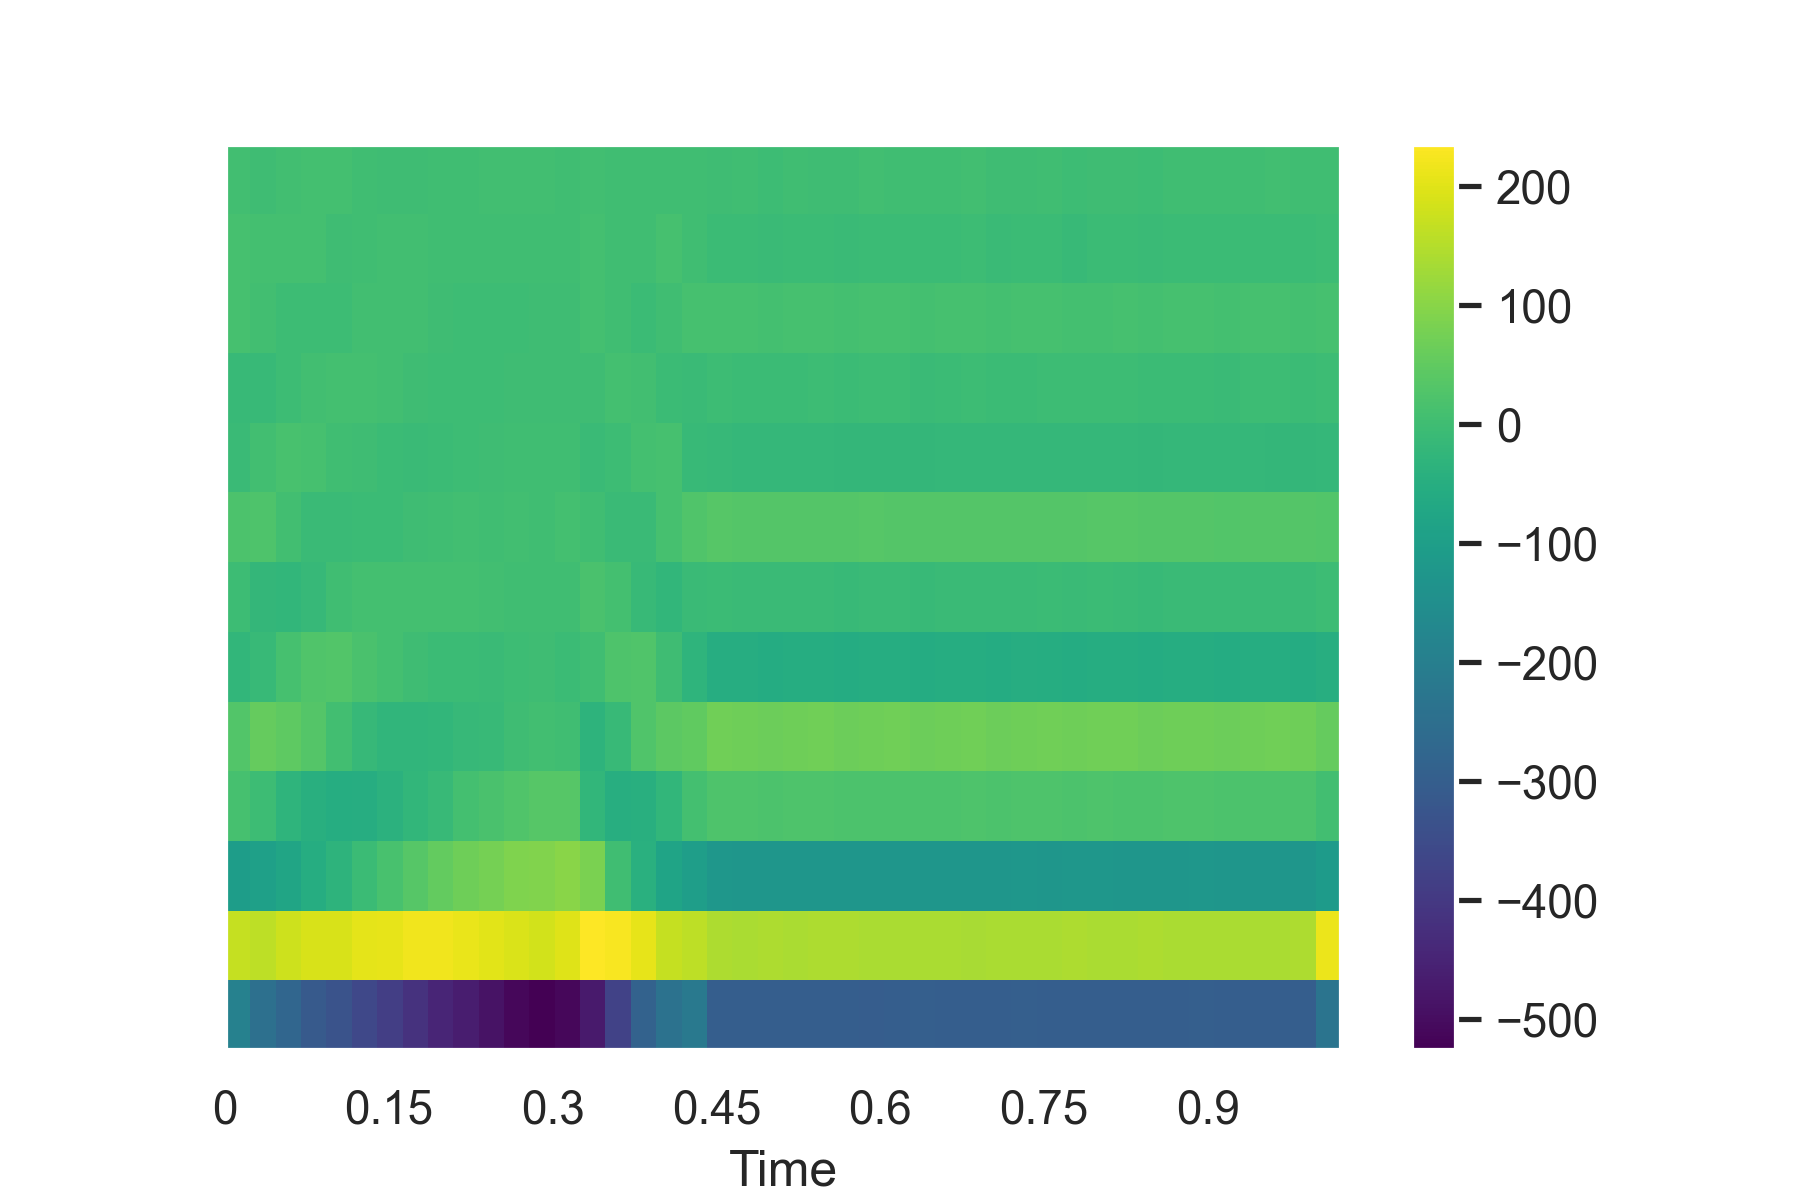
\includegraphics[width=\textwidth]{figures/inverse-synth/features_mfcc_example.png}
        \caption{MFCC}
    \end{subfigure}
    \begin{subfigure}[b]{0.45\textwidth}
        \centering
        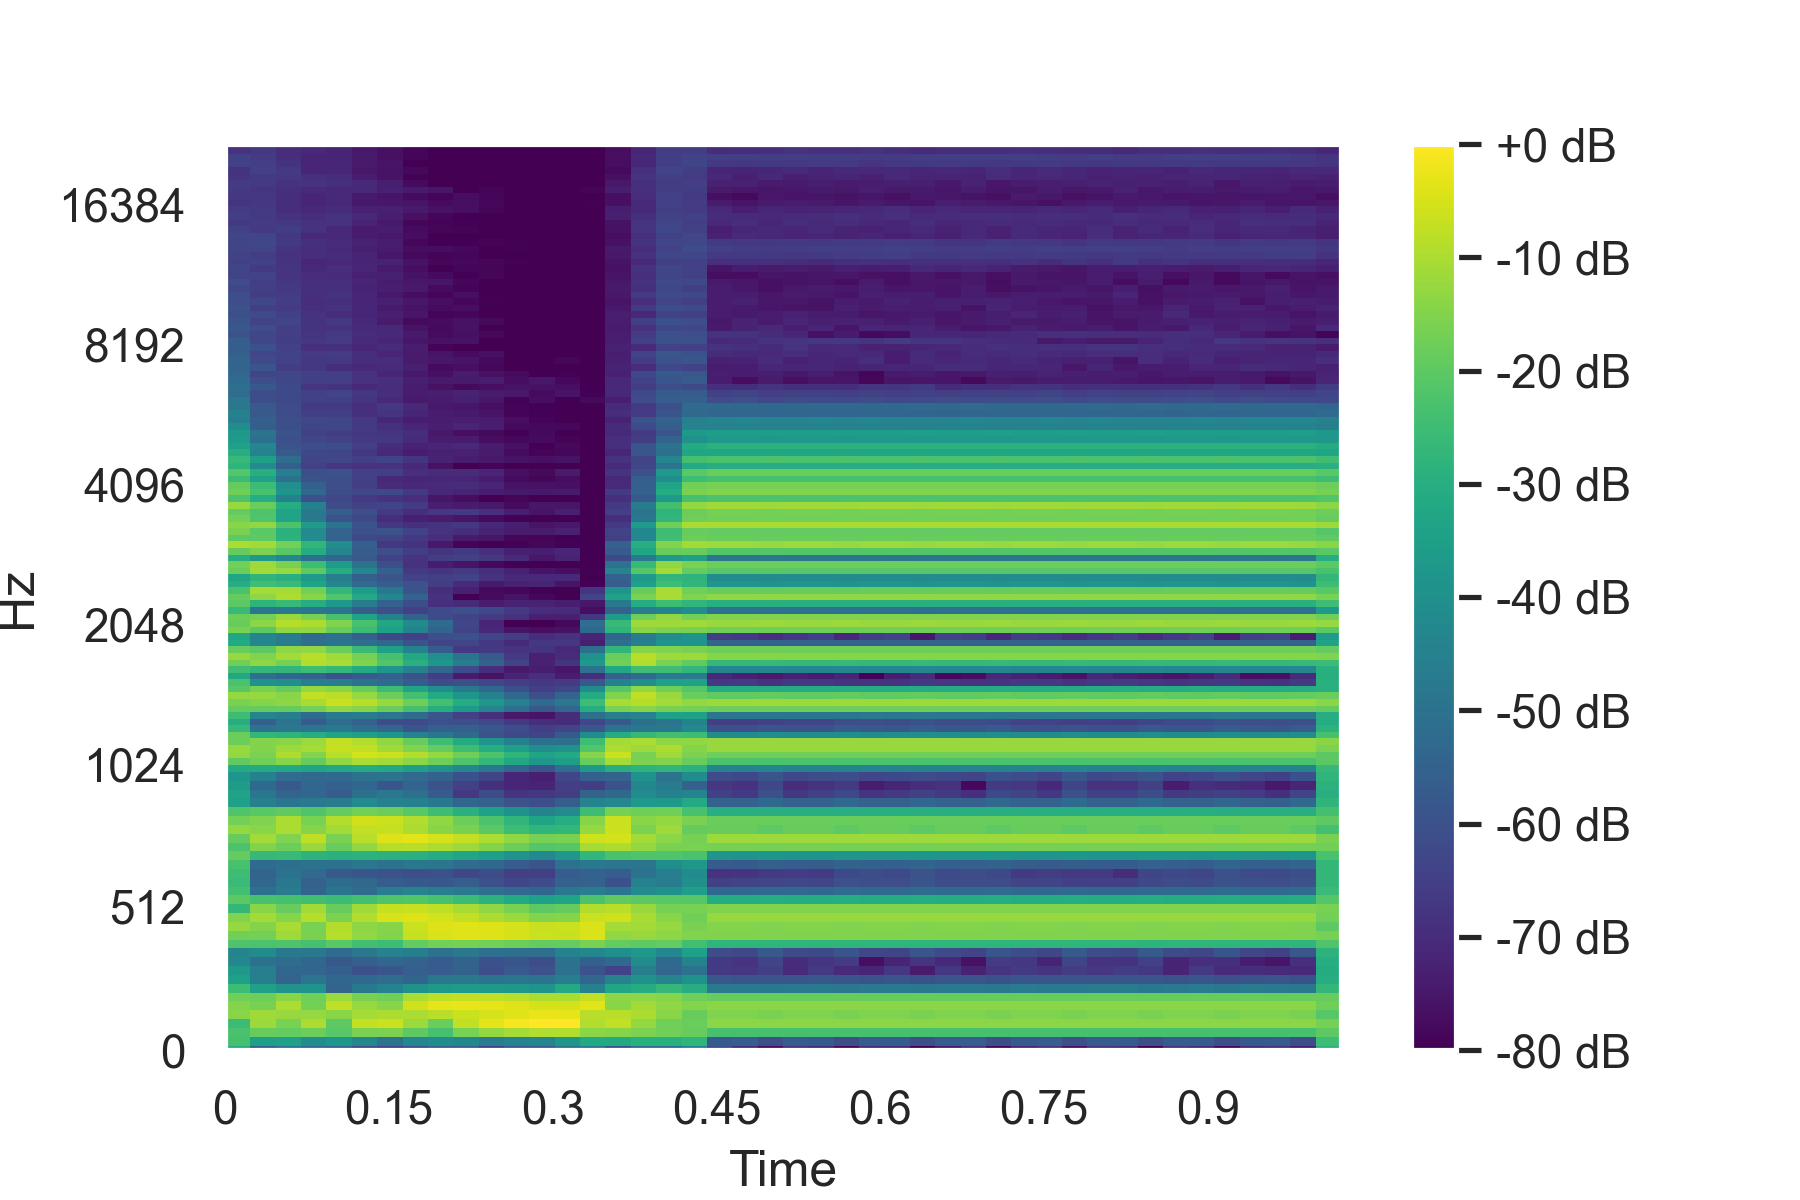
\includegraphics[width=\textwidth]{figures/inverse-synth/features_mel_example.png}
        \caption{Mel-Spectrogram}
    \end{subfigure}
    \caption{Audio representations generated for a single audio example in the dataset. The left figures shows a 13-band MFCC, and the right shows a log-scaled 128-band Mel-Spectrogram.}
    \label{fig:mfcc-mel-representations}
\end{figure}

\section{Deep Learning Models}
Four different models were used in this experiment. Two recurrent neural networks (RNNs) derived from work by Yee-King \textit{et al.} \cite{yee2018automatic}, a convolutional neural networks (CNNs) derived from work by Barkan \textit{et al.} \cite{barkan2019inversynth}, and a baseline multi-layer perceptron (MLP) network, also from Yee-King \textit{et al.} \cite{yee2018automatic}. Two versions of each of these models was created and optimized for either the MFCC or the Mel-spectrogram representation as input. All models output floating point value estimations for the seven synthesizer parameters. Because these output values can be any 32-bit floating point number (outputs are clipped to a $[0-1]$ range), this means that the models are solving a regression problem. The loss function used during training was the mean squared error (MSE) between the target parameter values $\textbf{y}$ and the predicted parameter values $\hat{\textbf{y}}$. The MSE is calculated as follows, where $N$ is the number of parameters:

\begin{equation}\label{equation:mse}
    \ell(\textbf{y}, \hat{\textbf{y}}) = \frac{\sum_{i \in N}{(y_i - \hat{y_i})^2}}{N}
\end{equation}

Ideally the loss would be calculated on audio produced by Dexed using the estimated parameters, however there are currently no available solutions for rendering audio using VST instruments within a deep learning model and including it in the the training loop. Recent work by Ramírez \textit{et al.} presented a solution for including audio effect plugins within a deep learning networks \cite{ramirez2021differentiable} which could also enable training on VSTis as well, however I leave that for future suggested work. 

Models were trained using an $Adam$ optimizer \cite{kingma2014adam} and hyperparameters for each model were optimized using a  Tree-structured Parzen Estimator (TPE), which has been shown to be an effective method for hyperparameter selection \cite{bergstra2011algorithms}. Early stopping was used during training for all models, this halted training if the validation loss stopped decreasing for over ten epochs.

The following subsections describe each of the models that were included in this experiment. To find specific details on the implementation of each model see appendix \ref{appendix:spiegelib_models} and for details on the hyperparameters used for training each model see [ADD THIS APPENDIX].

% Maybe not important
%This is a natural way to approach the problem considering the continuous nature of the parameters exposed by a given synthesizer, and this is the approach taken by Yee-King \textit{et al.}. Conversely, Barkan \textit{et al.} framed the inverse synthesis problem as a classification problem by dividing each parameter into 16 classes, which meant that there would be $n*16$ classes, where $n$ is the number of parameters. Quantizing the parameter space into 16 discrete values per parameter 

\subsection{Multi-Layer Perceptron}
% Find cites for  the MLP?
Multi-Layer Perceptron (MLP) models, also referred to as a feedforward neural network, were the first and most simple types of neural networks. They contain one or more hidden layers containing neurons that are connected to each neuron in the preceding and proceeding layers. Because of fully connected nature of these layers, they are also referred to as dense layers. An MLP is included in this experiment as a baseline model to benchmark the other models against. The architecture for the MLP was derived from Yee-King \textit{et al.} \cite{yee2018automatic} and has three hidden layers containing 256, 128, and 64 neurons respectively. Each neuron utilizes a ReLu activation. Dropout is included after the last hidden layer.

\subsection{Recurrent Neural Networks}
% Find cites for these different networks??
Two different Recurrent Neural Networks (RNNs) derived from work by Yee-King \textit{et al.} \cite{yee2018automatic} were used in this experiment:
\begin{itemize}
    \item \textit{LSTM:} The first is an RNN with three LSTM layers followed by a dropout layer and a fully connected linear output layer. The models used with MFCC input contained 64 units in each LSTM layer and the model used with Mel-spectrogram input had a larger capacity with 128 units in each LSTM layer.
    \item \textit{LSTM++:} The LSTM++ is a novel architecture proposed by Yee-King \textit{et al.} that performed the best on on their sound matching experiment \cite{yee2018automatic}. It features a bi-directional LSTM layer followed by a dropout, then a dense layer with an ELU non-linearity prior to several highway layers. In this experiment the size of the LSTM layers and the size and number of highways layers was selected using TPE. The models for MFCCs and Mel-spectrograms were the same and used LSTM layers with 128 units and seven highways layers each of size 128.
\end{itemize}

\subsection{Convolutional Neural Networks}
Barkan \textit{et al.} experimented with seven different CNN models for inverse synthesis that used a log STFT spectrogram input \cite{barkan2019inversynth}. They found that the model with the most capacity, a model with 6 CNN layers and 2.3M trainable parameters, performed the best in their experiments. All the other spectrogram based models that they experimented with had 1.2M trainable parameters and had between one to six convolutional layers. They also use strided convolutions as opposed to the more traditional max pooling approach to downsample between layers \cite{goodfellow2016deep}.

The 6-layer and 5-layer networks proposed by Barkan \textit{et al.} were implemented for this experiment. Early tests showed that these models were prone to overfitting and a derivative model with less capacity was developed for this experiment. This model had five convolutional layers with fewer filters in each of the layers to reduce the number of trainable parameters, which was found to help prevent overfitting.

The final CNN architecture that was selected for the MFCC model also included batch normalization between each of the convolutional layers and two fully-connected layers before the output, each with 512 neurons and ReLu activation. The Mel-Spectrogram CNN did not use batch normalization and had three fully-connected layers before the output, each with 128 neurons and ReLu activation. Both the CNNs had dropout before the fully-connected hidden layers. Figure \ref{fig:conv5s} shows a diagram of the Conv5s architecture used for the Mel-spectrogram inputs, excluding the batch normalization and dropout layers.

\begin{figure}[ht]
    \centering
    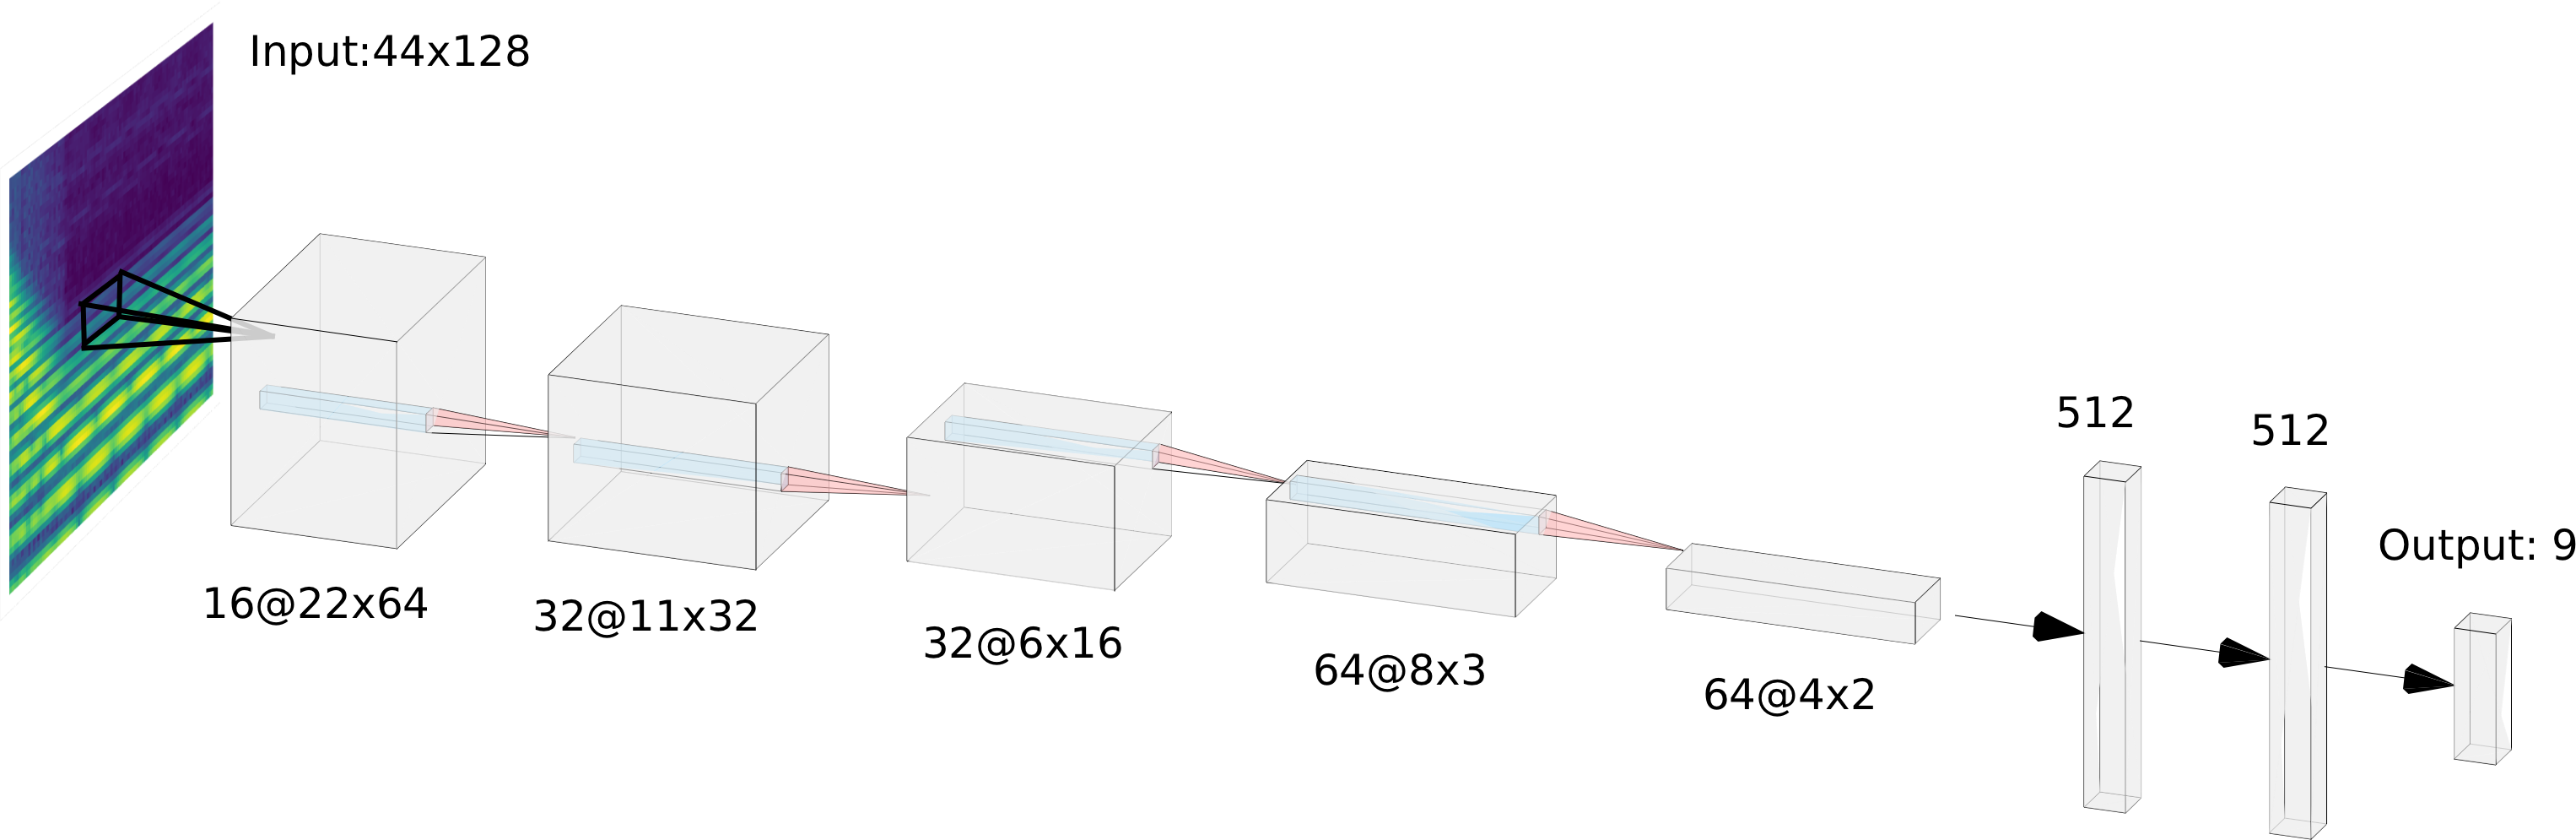
\includegraphics[width=0.99\textwidth]{figures/inverse-synth/CONV5s_Diagram.png}
    % Add a bit more description in this figure
    \caption{Network diagram of the CNN. This model accepts a Mel-spectrogram as input and contains five 2D convolutional layers followed by three dense layers. The output layer is predicted synthesizer parameters.}
    \label{fig:conv5s}
\end{figure}

Initial experiments showed that even the reduced capacity CNN was prone to overfitting. An inverse time-decay learning rate scheduler was introduced in an attempt to address this to allow the models to train for longer. The learning rate at each training step was defined by the following equation:

\begin{align}
    \eta_i = \frac{\eta_0}{1 + \lambda\frac{i}{T}}
\end{align}

Where $\eta_i$ is the learning rate at training step $i$, $\eta_0$ is the initial learning rate, $\lambda$ is the decay rate, and $T$ is the decay steps. For this experiment $\eta_0=0.001$ and $T$ was set to be equivalent to 25 epochs. $\lambda=3$ for the MFCC CNN and $\lambda=4$ for the Mel-Spectrogram CNN.

\subsection{Training Results}
All the models were allowed to train until the early-stopping criteria was triggered. The number of training epochs ranged from 31 epochs for the Mel-LSTM to 133 epochs for the Mel-MLP.
% Maybe include this?
%Models were trained on an NVIDIA RTX 2080 super GPU, training time ranged between X for the X model, and Y for the Y model. All training times are listed in appendix \ref{appendix:training-times}.
Validation loss at each training epoch is shown in figure \ref{fig:training-loss} and plots for all models plotted against their respective training loss are provided in appendix \ref{appendix:training-loss}. The MFCC-LSTM and MFCC-LSTM++ models achieved the lowest validation loss during training, $\approx 0.042$. All the MFCC versions of the models achieved better final validation loss values when compared their Mel-Spectrogram counterparts, although only by a small amount; the average final loss for MFCC models was 0.044 whereas the average final loss for the Mel models was 0.045.
\begin{figure}[ht]
    \centering
    \begin{subfigure}[b]{0.49\textwidth}
        \centering
        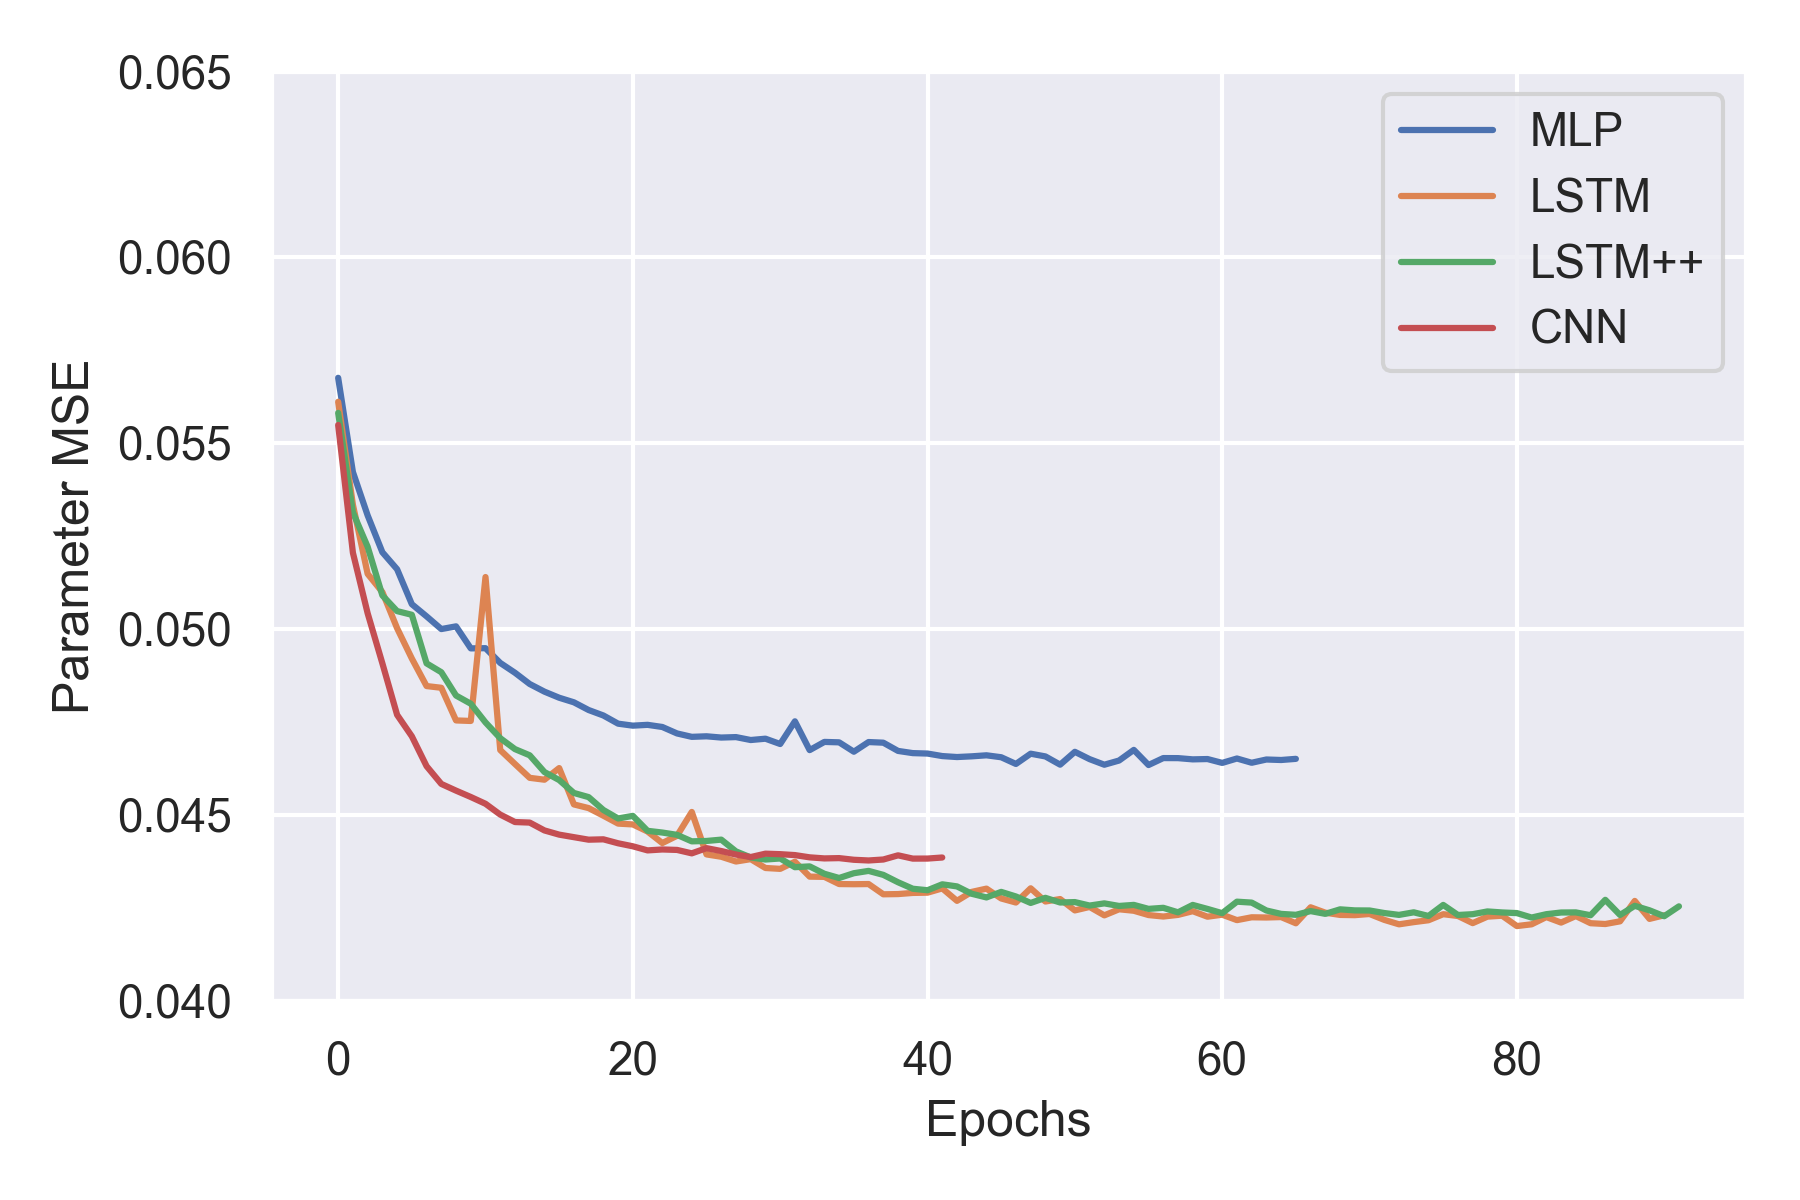
\includegraphics[width=\textwidth]{figures/inverse-synth/mfcc-model-loss.png }
        \caption{MFCC Models}
    \end{subfigure}
    \begin{subfigure}[b]{0.49\textwidth}
        \centering
        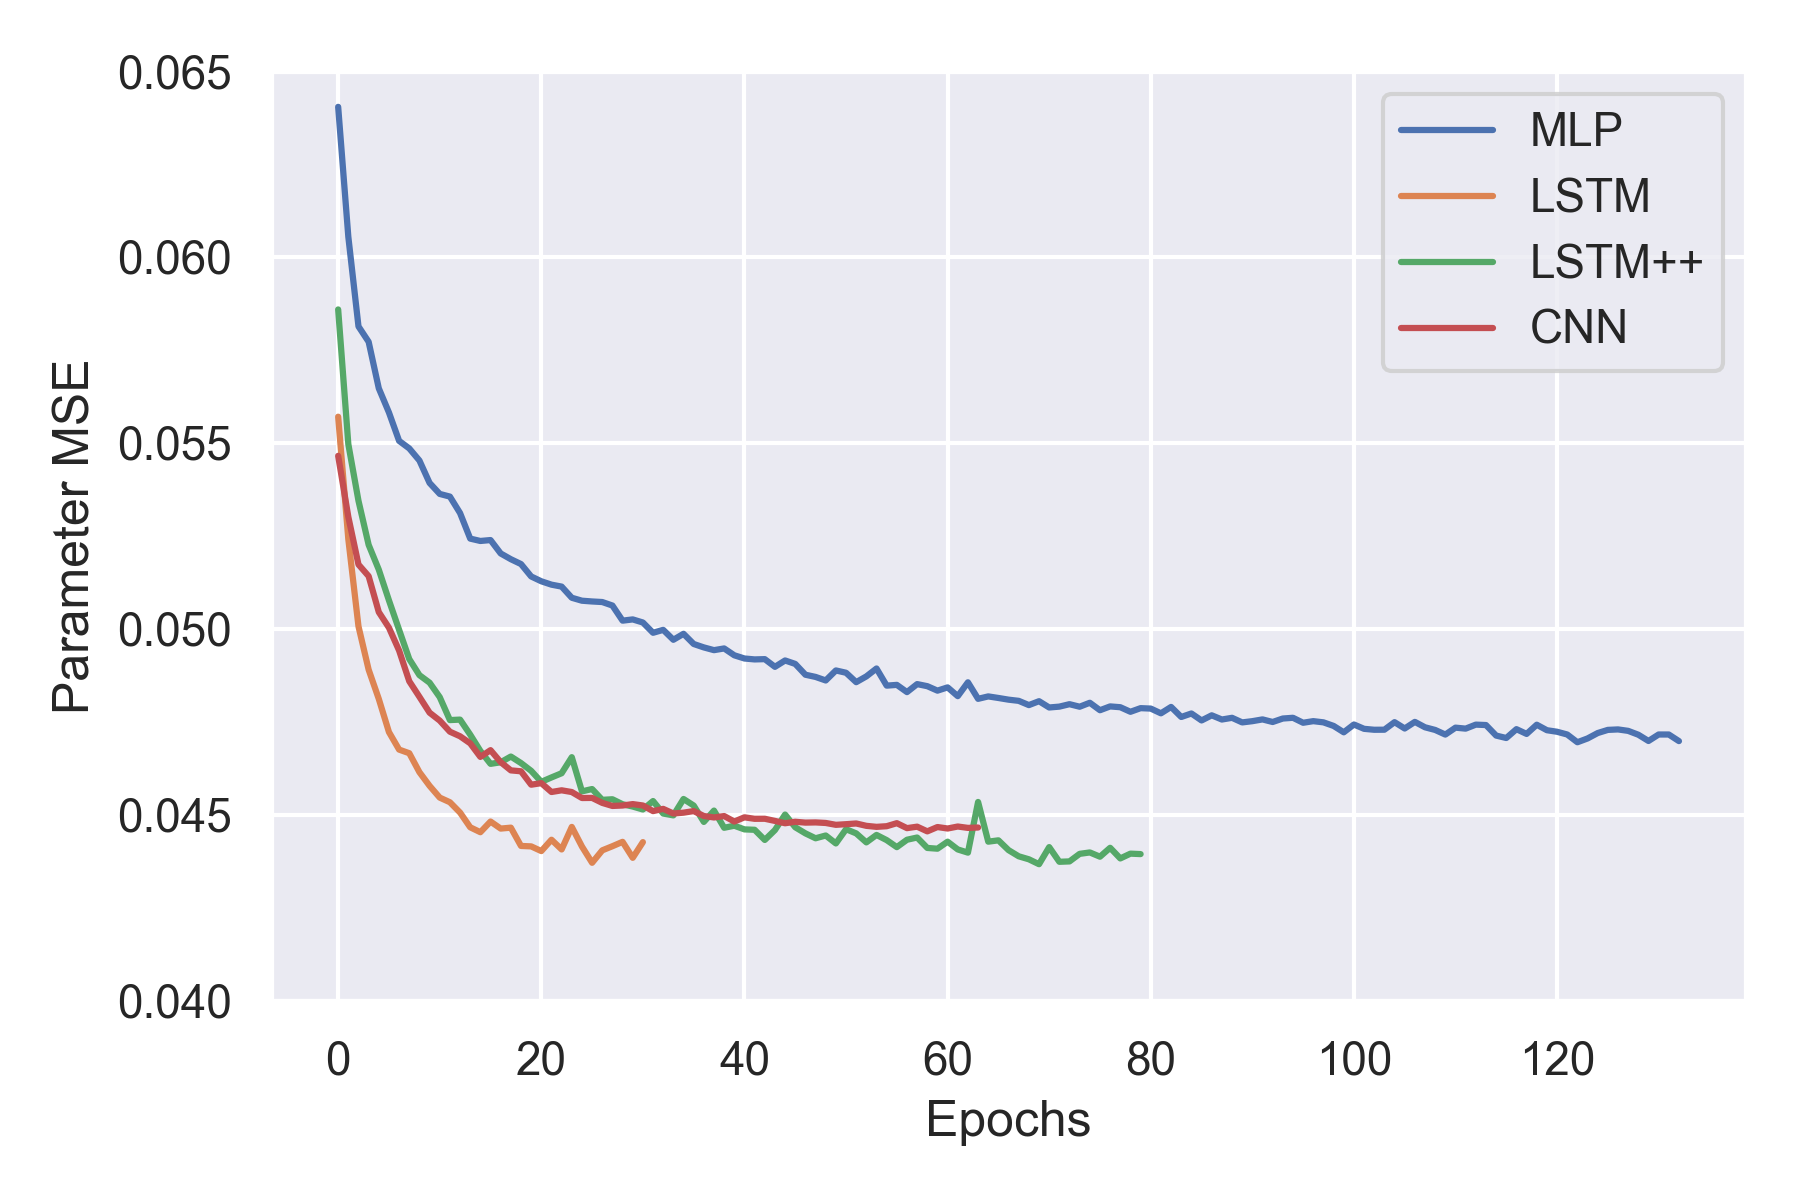
\includegraphics[width=\textwidth]{figures/inverse-synth/mel-model-loss.png}
        \caption{Mel-Spectrogram Models}
    \end{subfigure}
    \caption{Validation loss during training for all the deep learning models.}
    \label{fig:training-loss}
\end{figure}

\section{Genetic Algorithms}
\label{inverse-synth:ga}

Two different GAs were used: a basic single-objective GA and a multi-objective NSGA III. The multi-ojective GA was derived from work conducted by Tatar \textit{et al.} \cite{tatar2016automatic} that used the algorithm to automatically tune the parameters of a Teenage Engineering OP-1\footnote{\url{https://teenage.engineering/products/op-1}} synthesizer. In the case of the GAs the $fitness$ is easily computed directly on the audio rendered from $Dexed$. During each iteration of the algorithm, individuals of the population (whose genotype are synthesizer parameters) are rendered using Dexed, and the phenotype is produced by generating an audio representation from the resulting audio.

\subsection{Fitness}
In the case of the basic GA, the $fitness$ is computed as the mean absolute error (MAE) between 13-band MFCCs from the target and the individual. The MFCCs were calculated using a frame-size of 2048 samples and a hop-size of 1024 samples. MAE is calculated as follows, where $N$ is the number of features, $y$ is the target, and $\hat{y}$ is the predicted individual:

\begin{equation}\label{equation:mae}
    \text{MAE} = \frac{\sum_{i \in N}{|y_i - \hat{y}_i|}}{N}
\end{equation}
 
 Three different metrics were used for evaluating the $fitness$ of an individual for the NSGA-III algorithm, MAE between: 1) a 13-band MFCC, 2) magnitude spectrum from an FFT, and 3) a set of spectral features. The MFCCs were calculated using a frame-size of 2048 samples and hop size of 1024 samples. The FFT was calculated over the entire input audio, 1 second at 44,100 samples/second. For the spectral features, five different features were calculated: centroid, bandwidth, contrast across seven subbands, flatness, and rolloff. Each feature was calculated using a frame-size of 2048 samples and a hop-size of 1024 samples. The time series of audio features was summarized using the mean and variance. This resulted in a feature vector of size 22.
 
 \subsection{Generations}
 The quality of the result that can be produced by a GA is generally related to the amount of time that the algorithm is allowed to run for. While there is no guarantee that the optimal solution will be found, and the optimization may get stuck in a local minima, allowing the the algorithm to run for longer gives a higher likelihood of finding a quality solution. Tatar \textit{et al.} allowed their NSGA-III run for 1000 generations, which took 5 hours on a 50-core computer. The results of their method where competitive with an experienced human sound designer. 
 
 The synthesizer programming task in their problem was much more complex than the problem presented in this experiment. Initial experiments showed both GAs were able to perform well when allowed to run for 100 generations with a population of 300 individuals. For the NSGA this took about 20 minutes on a late-2013 MacBook Pro. Although this time is much better than 5hrs, this still limited the number of target examples that could be used for evaluation. 20 minutes is also a long time for application that is expected to be used in a music production context. 
 
 To experiment with reducing the runtime of the GAs, a more severely constrained test was designed. Each GA was allowed to run for only 25 generations using a population of 100 individuals. These values were selected to significantly reduce the runtime and to validate whether competitive solutions could still be generated. With these constraints the runtime was approximately 75 seconds for the NSGA-III and 41 seconds for the basic GA when predicting parameters for a 1 second long target audio.
 
 \subsection{Mutation and Crossover}
 The remaining hyperparameters that control each GA are the rate of mutation and the rate of crossover. The rate of mutation sets the likelihood that a genotype is randomly modified. The rate of mutation was 30\% for the basic GA and 50\% for the NSGA-III. Rate of crossover set the likelihood that an individual is combined with another individual to create an new "child" individual. The rate of crossover for both GAs was set to 50\%.


% Both genetic algorithms were run for 100 generations for each sound target. The basic GA and NSGA used population sizes of 300 and 100 individuals respectively. 

%Figure \ref{fig:nsga_fitness} shows the minimum spectral error achieved by an individual during each iteration of the NSGA algorithm on one of the target sounds. The plot shows a period of rapid improvement during early iterations, with some short periods of stagnation, followed by longer periods where the algorithm is unable to find an individual that is an improvement over those in the current population.

% TODO: Add in the other population generation plots for each objective

% \begin{figure}[ht]
% \begin{center}
% 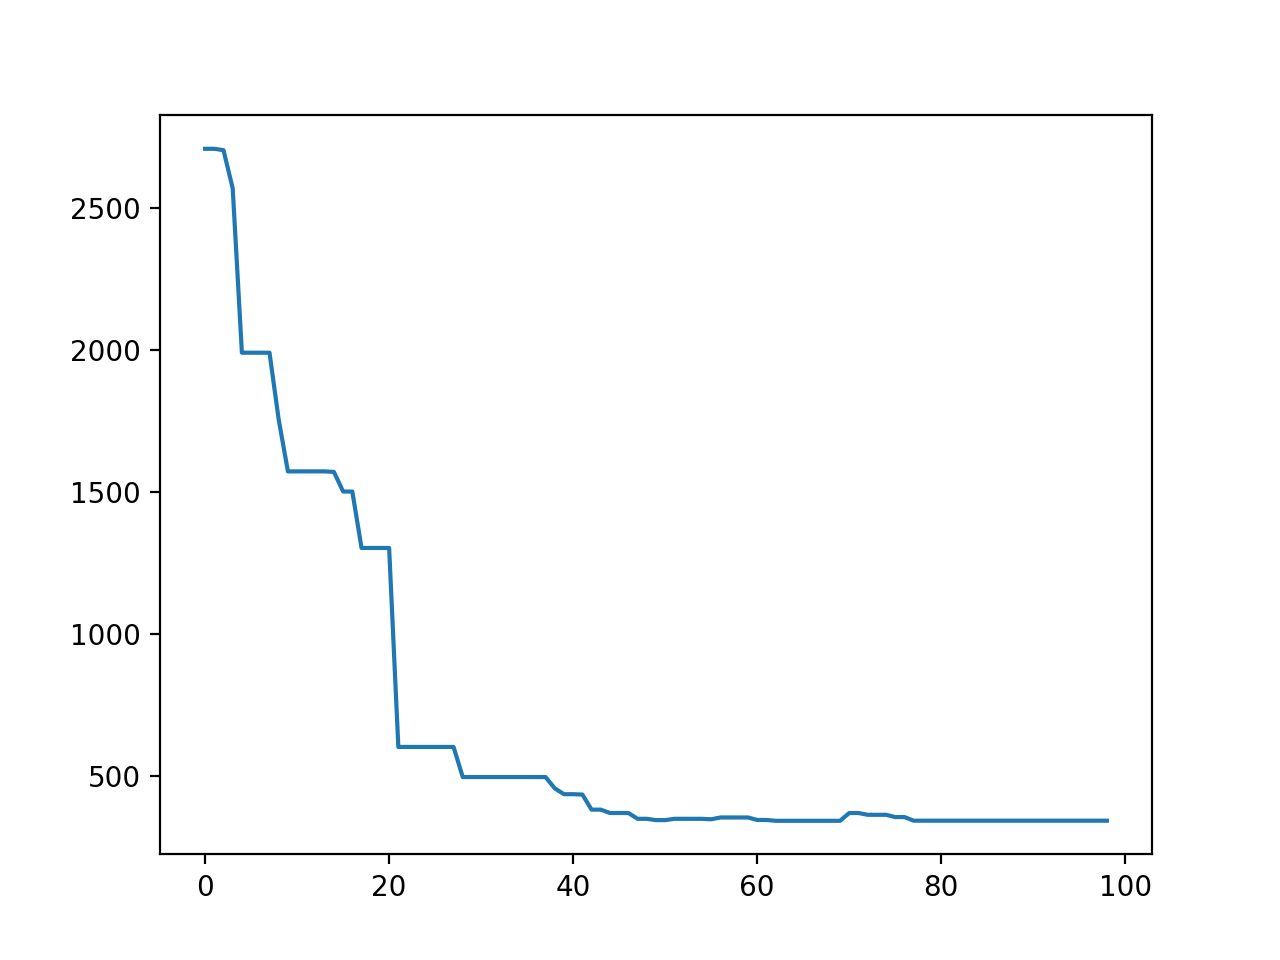
\includegraphics[width=0.7\columnwidth]{nsga_target_15_FFT.png}
% \caption{Minimum FFT MAE in the population at each generation to target sound 15 for NSGA III estimator.}
% \label{fig:nsga_fitness}
% \end{center}
% \end{figure}
\subsection{Warm Start Genetic Algorithm}
A novel hybrid method that combines the strengths of deep learning and genetic algorithms was developed for this experiment. Deep learning models front-load the computational  complexity during model training, which can take several minutes to several hours, however are comparatively fast during parameter prediction (less than 100ms for the models included in this experiment). However, deep learning approaches have yet to achieve the same accuracy and consistency as genetic algorithms for parameter estimation.

The method proposed here leverages the inference speed of deep learning models to support the generation of the initial population for a NSGA-III. This gives the the genetic algorithm a head start during optimization instead of starting with a population of purely random solutions. Because of this, the method is called \textit{Warm-Start NSGA} or \textit{WS-NSGA} for short.

To generate the initial population, parameters are first predicted using a pre-trained model. The MFCC-LSTM++ model was selected based on results presented in the following section. This produces a single individual for the population. Forty nine mutated versions of this individual are generated and added to the population. Finally, to add variation to the population another fifty random individuals are created. The algorithm is then run exactly the same as the regular NSGA, however now with only ten generations. This method takes approximately 30 seconds in total per prediction.

\section{Evaluation}
\label{sec:inverse-synth-eval}

Evaluation was carried out by measuring the ability of each technique to accurately perform inverse synthesis on a set of 250 testing sounds. The same seven parameter subset of sounds were used for the test dataset, this means that an exact match for inverse synthesizer is possible, which provides a known baseline for comparing each of the methods. Each of the 11 different techniques were were run on each of the 250 target test sounds and parameters estimated. The trained models for all the deep learning approaches were used for estimation and inference on a single target took $\approx 70$ms on Macbook Pro. The GAs were each run on each of the 250 target sounds, which took $\approx 5$ hours using the NSGA-III and $\approx 3$ hours with the basic GA, and $\approx 5$ hours using the WS-NSGA. 

%Figure \ref{fig:nsga-error-generations} shows an example of how the fitness values for the three objectives are optimized over consecutive generations. These figures illustrate how performance can vary significantly from target to target, both examples started with populations that contained individuals with relatively high error with respect to the objectives, the search for target 35 successfully found a solution with minimal error for all objectives, however the search for target 5 was only able to find a solution that resulted in low error for one of the objectives.
%
%\begin{figure}[ht]
%    \centering
%    \begin{subfigure}[b]{0.49\textwidth}
%        \centering
%        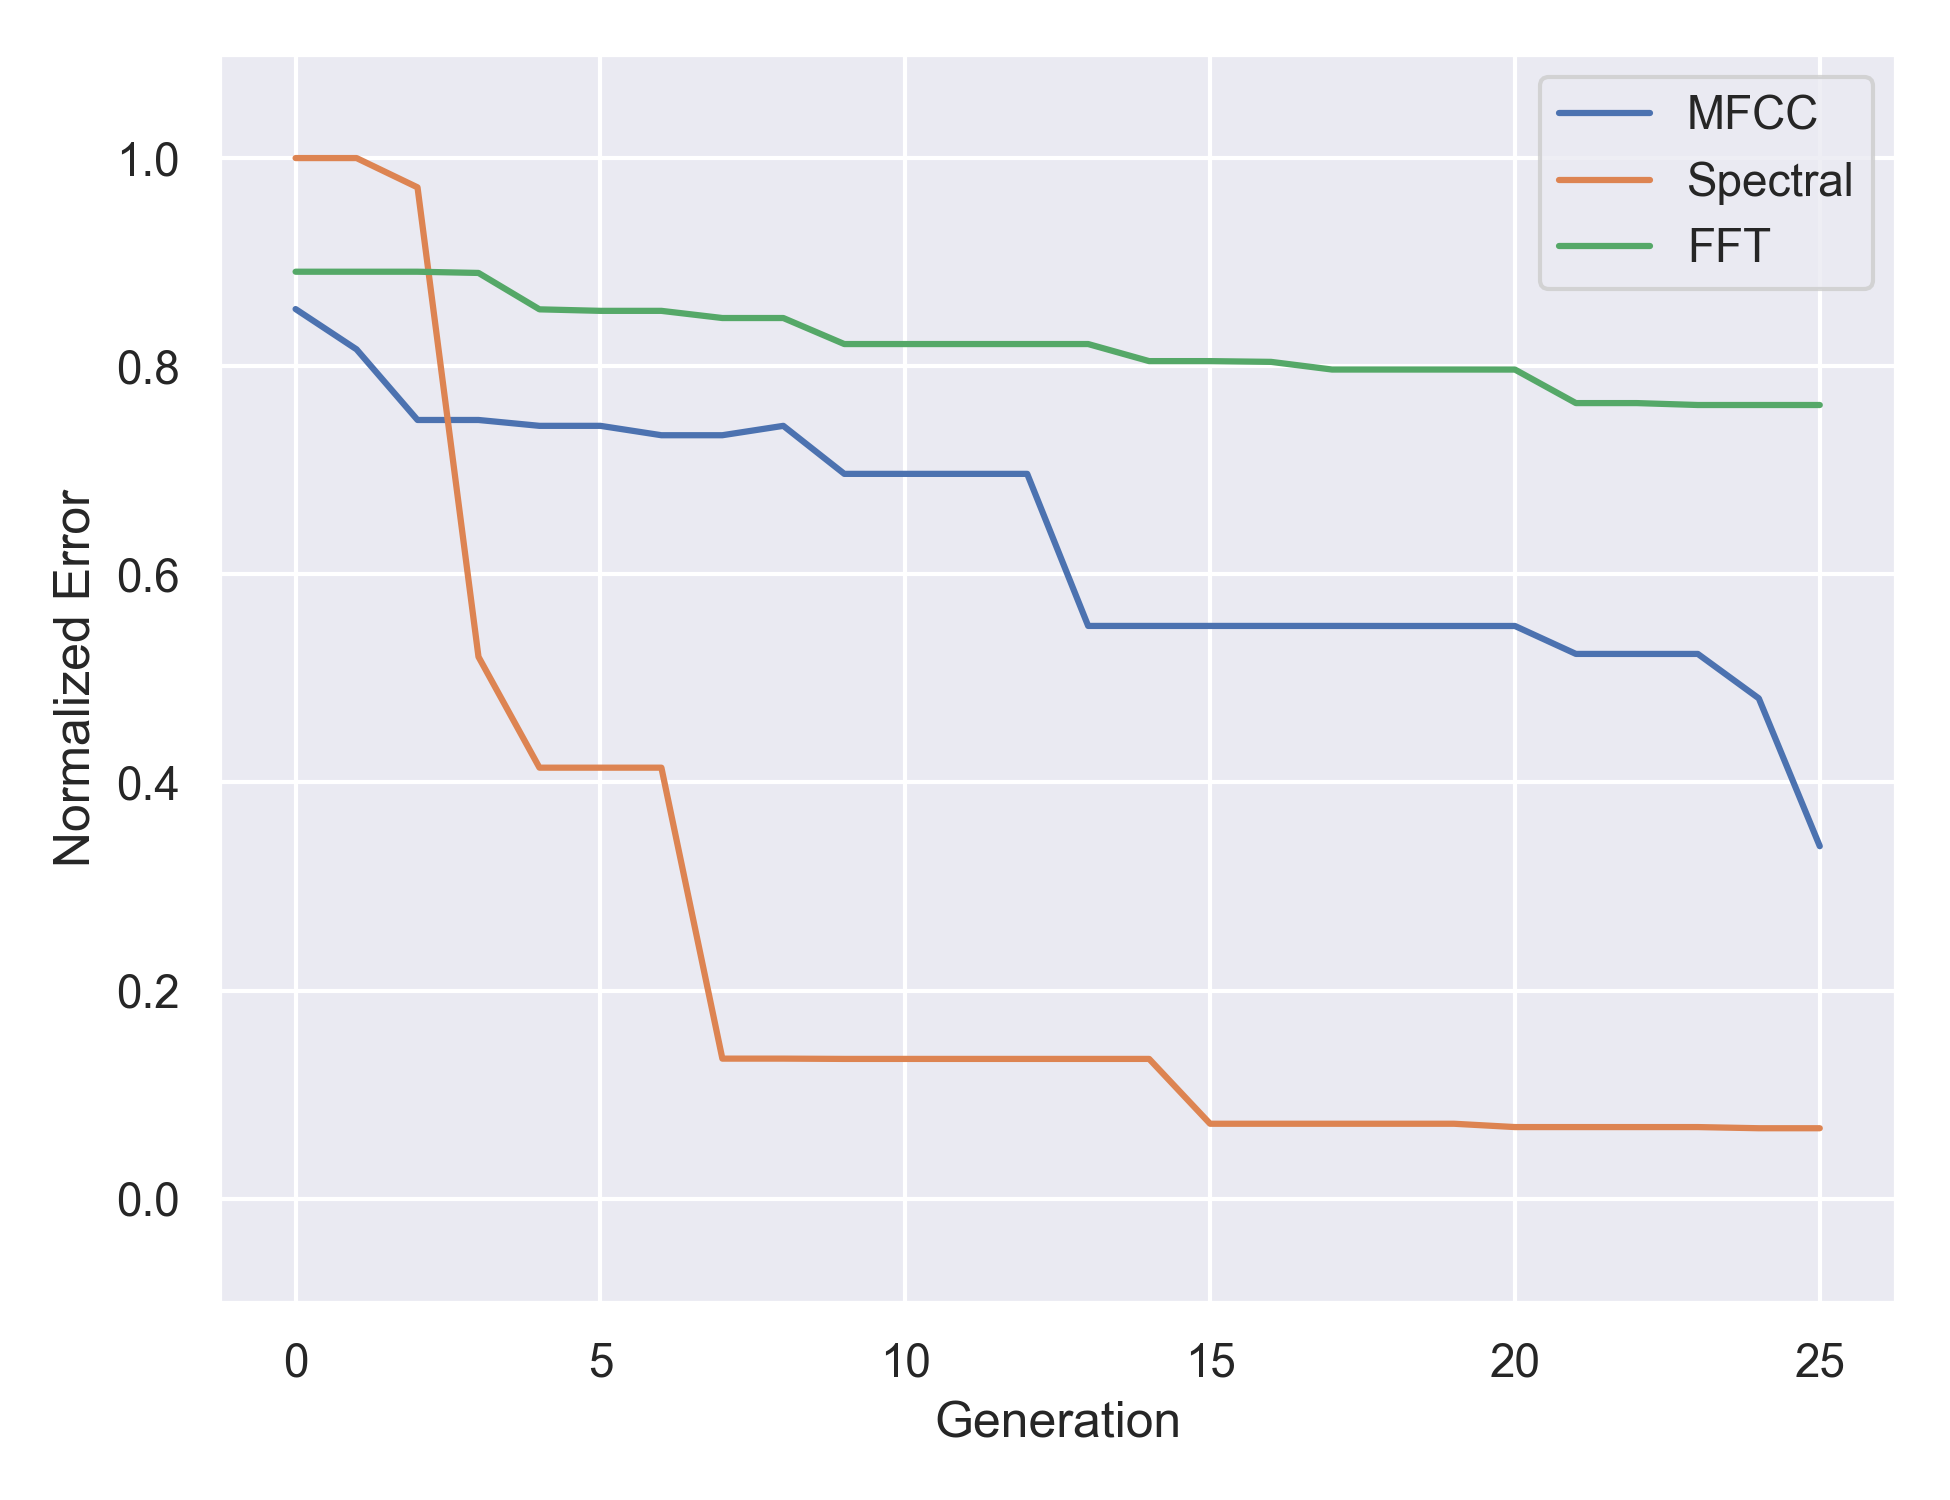
\includegraphics[width=\textwidth]{figures/inverse-synth/nsga_plot_5.png}
%        \caption{Target 5}
%    \end{subfigure}
%    \begin{subfigure}[b]{0.49\textwidth}
%        \centering
%        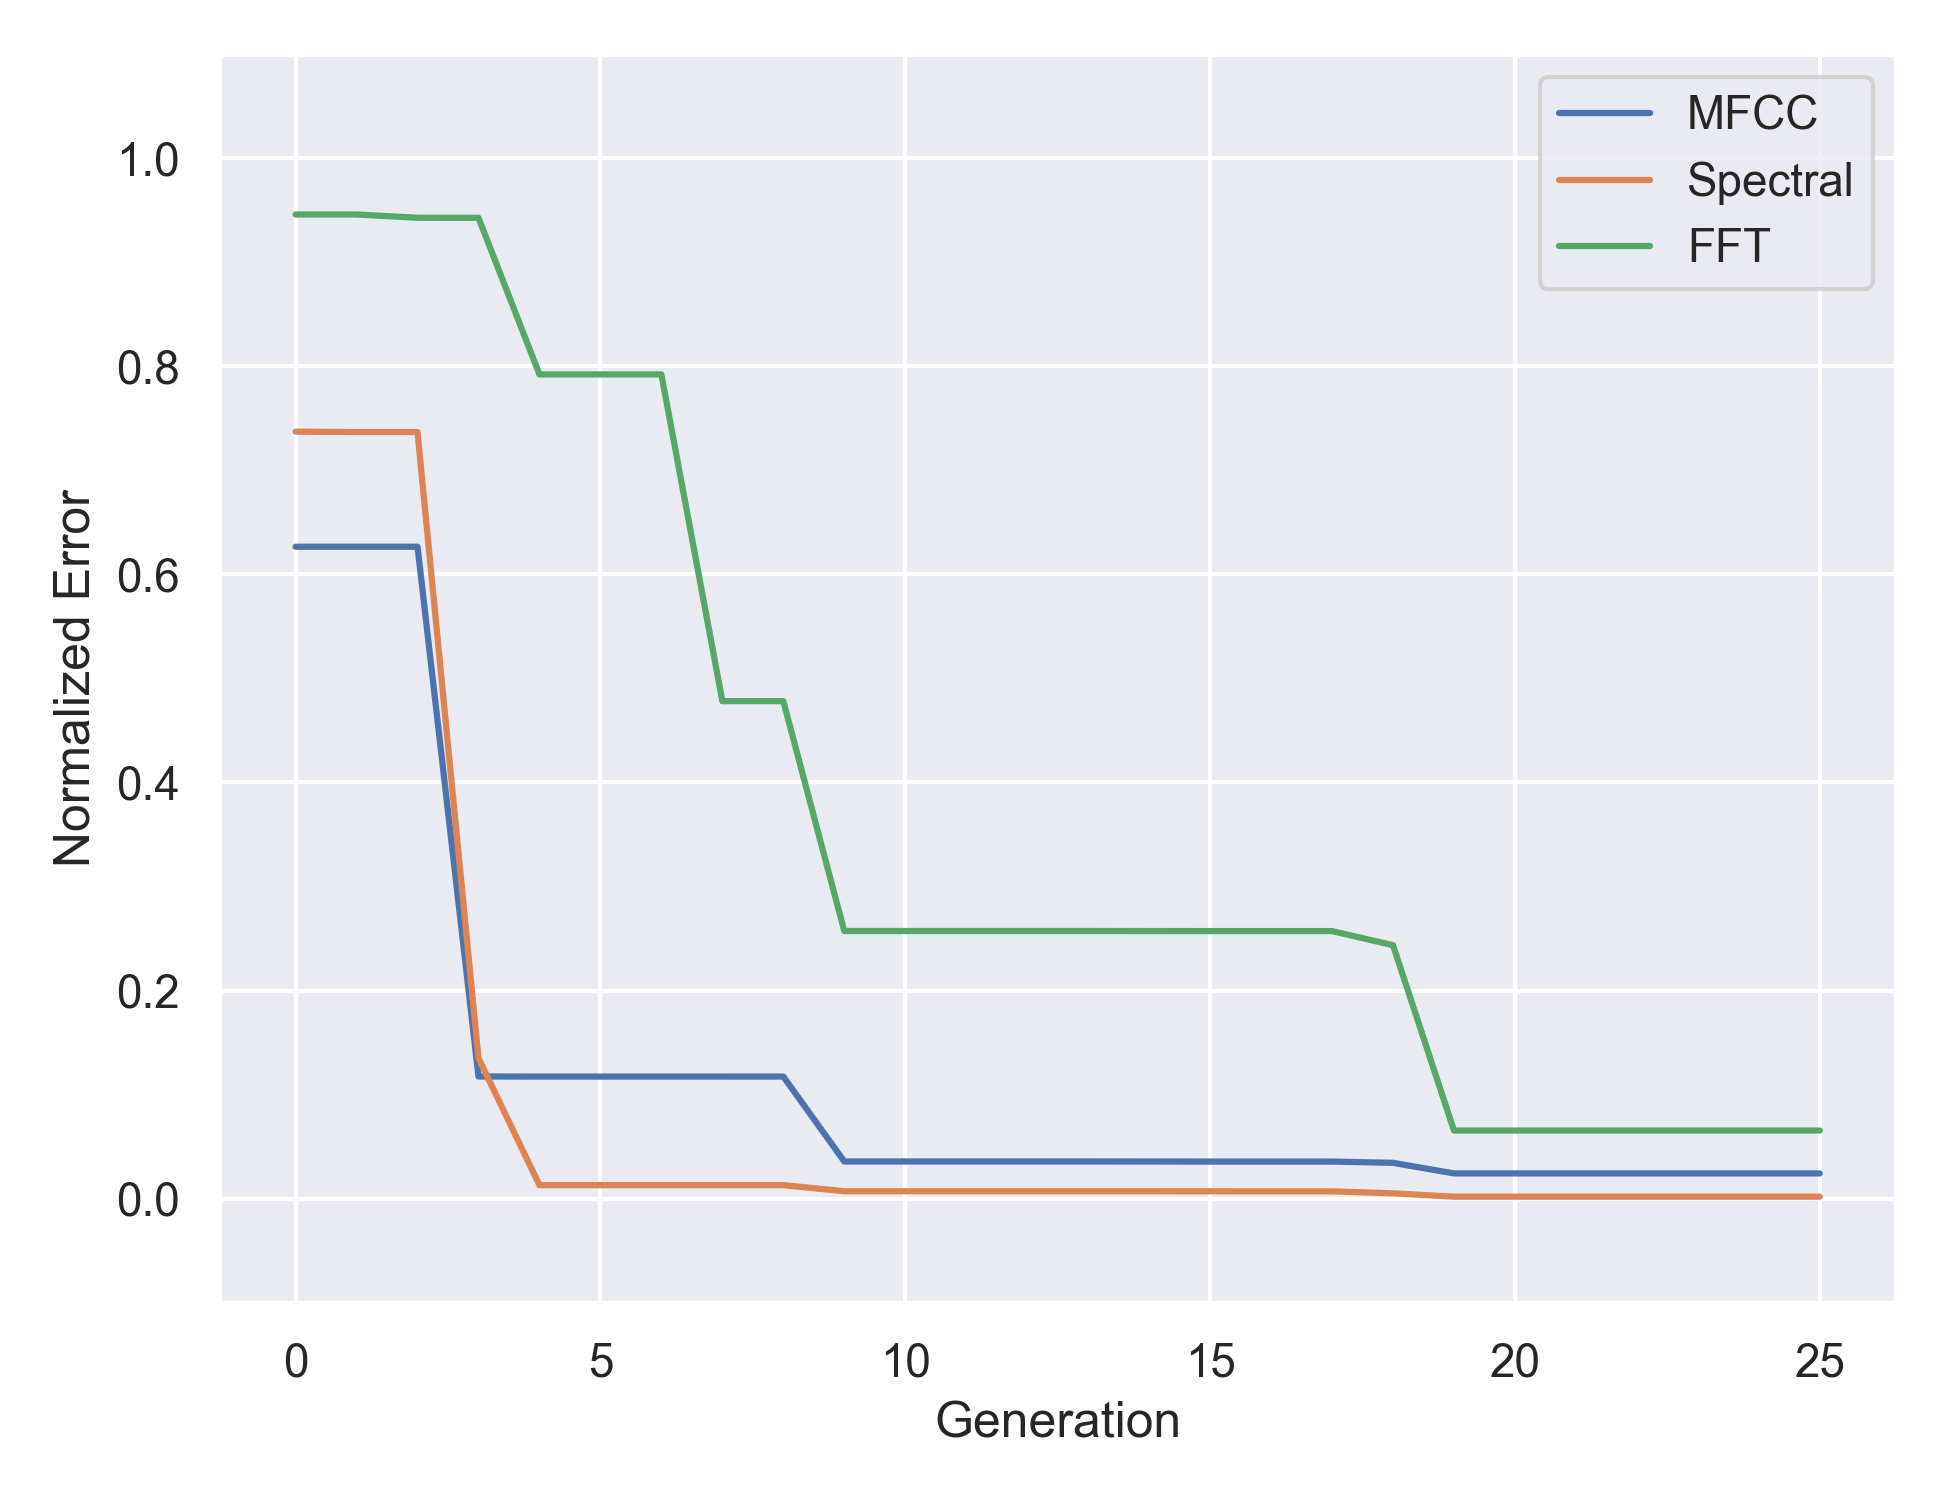
\includegraphics[width=\textwidth]{figures/inverse-synth/nsga_plot_35.png}
%        \caption{Target 35}
%    \end{subfigure}
%    \caption{Plots showing the minimum fitness values for each objective in the NSGA-III over generations during prediction for two examples from the testing dataset. Error for each objective was normalized using the maximum minimum fitness achieved over all testing trials.
%    % The left plot shows an example where the best individual in the population at the beginning of the search had high error with respect to the objectives, an example was found that improved the spectral error quite drastically, however the MFCC and FFT error remained high. The right plot shows an example where the algorithm was able to find an example that significantly improved all objectives.
%    }
%    \label{fig:nsga-error-generations}
%\end{figure}

Predicted audio was rendered using Dexed and the the resulting audio and parameter pairs were saved for evaluation. The results were evaluated quantitatively using three different metrics: 1) MFCC MAE,  2) Log Spectral Distance (LSD), 3) Parameter MAE. The first two metrics are calculated on the audio directly and the the third on the predicted parameters. Each metric is described in more detail below and all the results are summarized in table \ref{tbl:objective_resuls} and in box plots shown in figure \ref{fig:eval-boxplot}.

\begin{table}[ht]
\centering
\begin{tabular}{l|ccc}
\toprule
% {} & \multicolumn{2}{c}{MFCC MAE} & \multicolumn{2}{c}{LSD} & \multicolumn{2}{c}{Parameter MAR} \\
{} & MFCC & LSD & Parameter \\
\midrule
MFCC-MLP    &       $5.9 \pm      6.8$ &     $83.2 \pm    12.0$ &     $0.1615 \pm    0.0521$ \\
MFCC-LSTM   &       $4.0 \pm      4.9$ &     $80.1 \pm     9.1$ &     $0.1515 \pm    0.0579$ \\
MFCC-LSTM++ &       $4.1 \pm      3.9$ &     $79.9 \pm    10.2$ &     $\mathbf{0.1483 \pm    0.0552}$ \\
MFCC-CNN    &       $4.5 \pm      4.7$ &     $81.5 \pm    10.0$ &     $0.1501 \pm    0.0547$ \\
\midrule
Mel-MLP     &       $6.7 \pm      7.1$ &     $83.1 \pm    13.2$ &     $0.1686 \pm    0.0499$ \\
Mel-LSTM    &       $4.7 \pm      5.2$ &     $80.4 \pm    11.3$ &     $0.1524 \pm    0.0565$ \\
Mel-LSTM++  &       $4.8 \pm      4.8$ &     $81.4 \pm     9.7$ &     $0.1513 \pm    0.0536$ \\
Mel-CNN    &       $5.5 \pm      6.1$ &     $81.5 \pm    10.9$ &     $0.1569 \pm    0.0526$ \\
\midrule
GA          &       $4.0 \pm      3.0$ &     $81.2 \pm    11.3$ &     $0.2400 \pm    0.0881$ \\
NSGA        &       $1.4 \pm      2.5$ &     $\mathbf{72.5 \pm    27.3}$ &     $0.2120 \pm    0.0897$ \\
WS-NSGA     &       $\mathbf{1.3 \pm      1.8}$ &     $72.6 \pm    23.4$ &     $0.1511 \pm    0.0604$ \\
\bottomrule
\end{tabular}
\caption{Summary of quantitative results for inverse synthesis evaluation. The values in bold are the scores with the lowest mean for that metric.}
\label{tbl:objective_resuls}
\end{table}

\begin{figure}[p]
    \centering
    \begin{subfigure}[b]{0.99\textwidth}
        \centering
        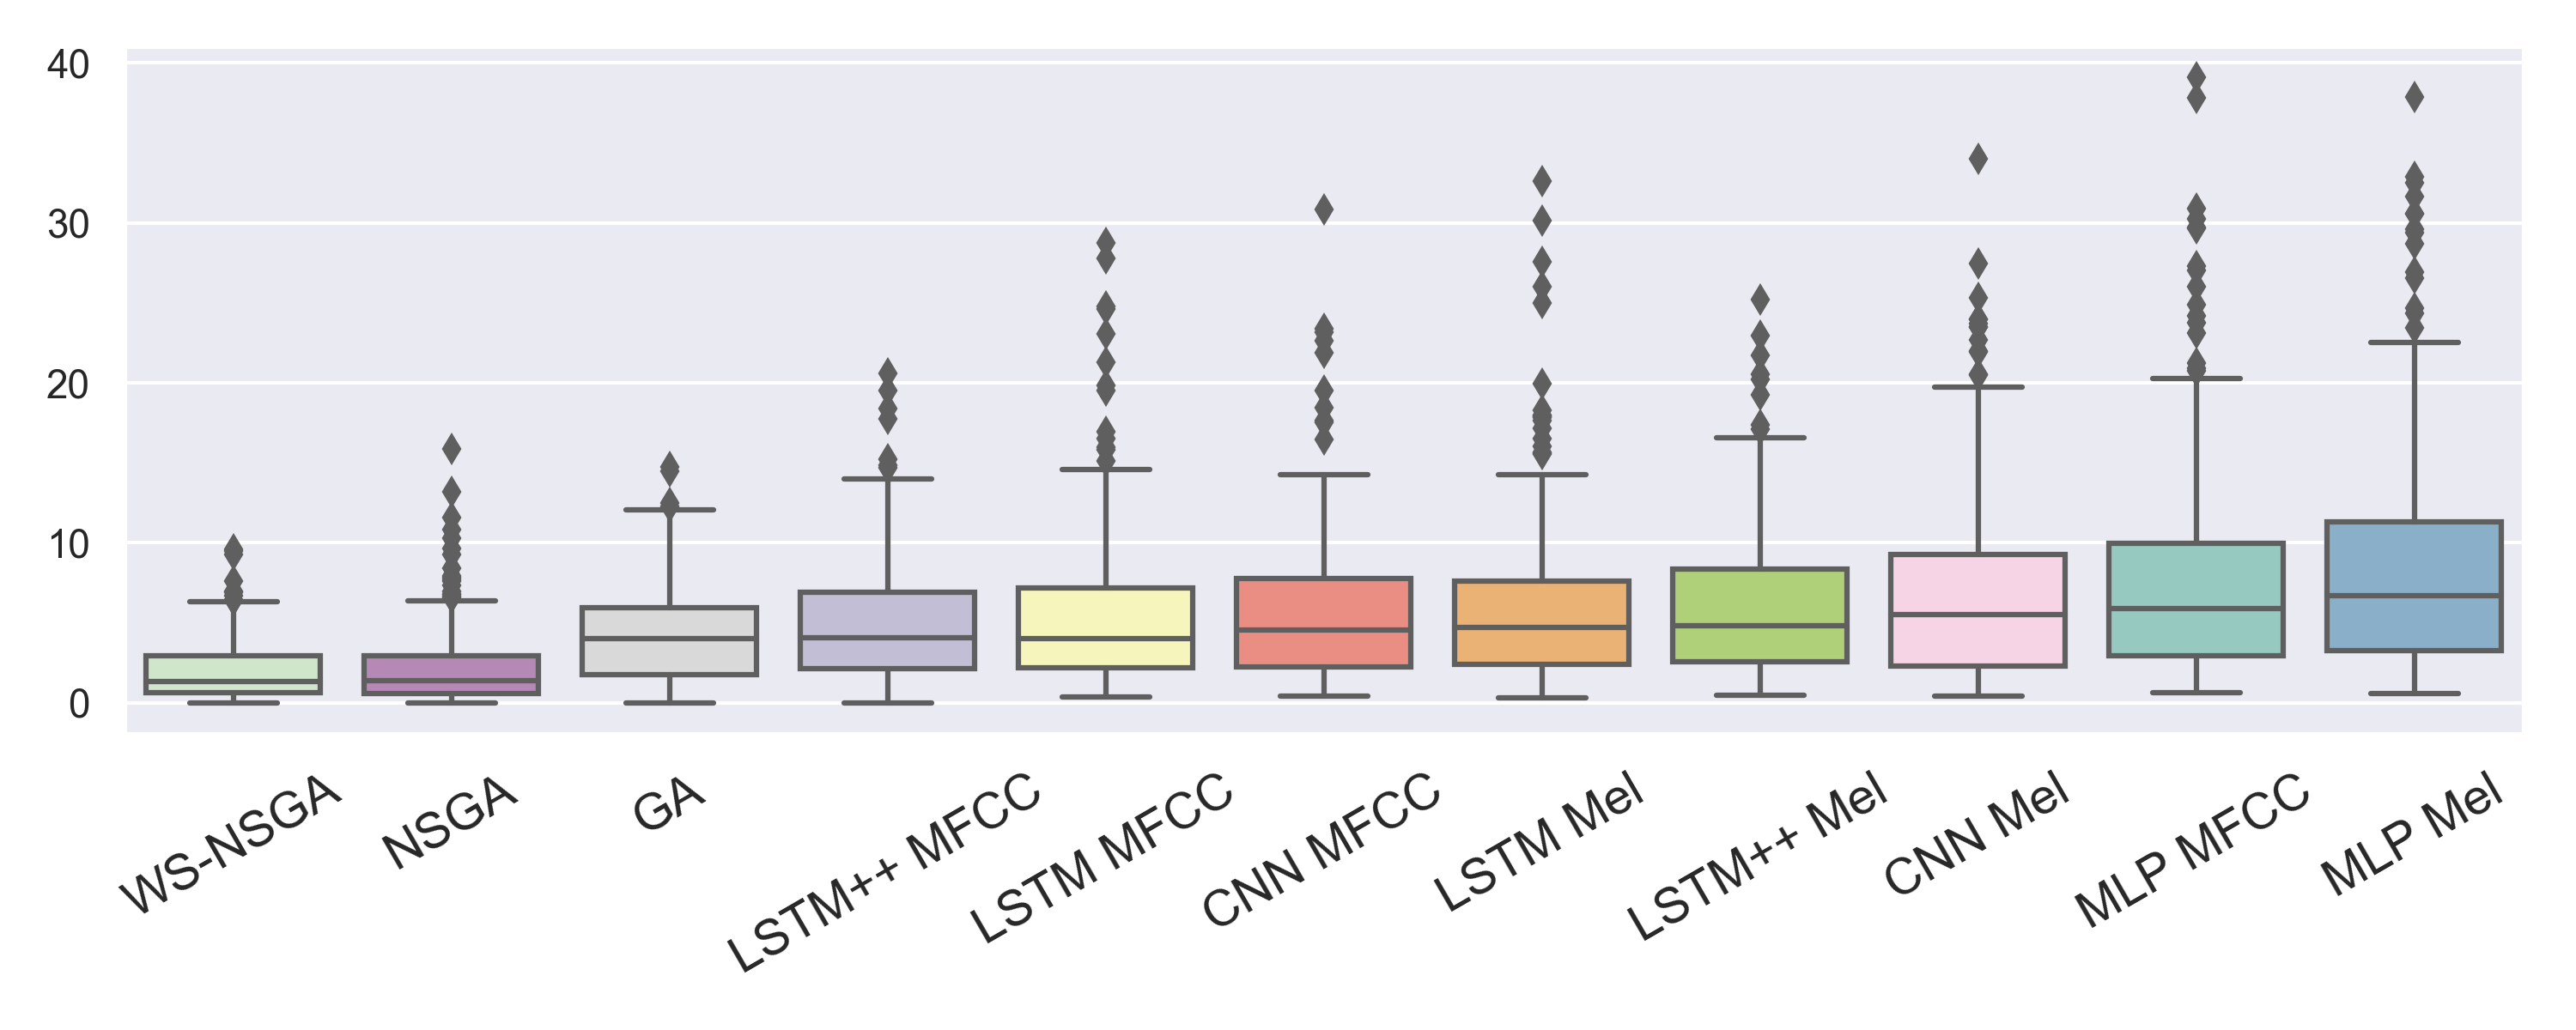
\includegraphics[width=\textwidth]{figures/inverse-synth/mfcc_mae_boxplot.png}
        \caption{MFCC MAE}
        \label{fig:mfcc-mae}
    \end{subfigure}
    \begin{subfigure}[b]{0.99\textwidth}
        \centering
        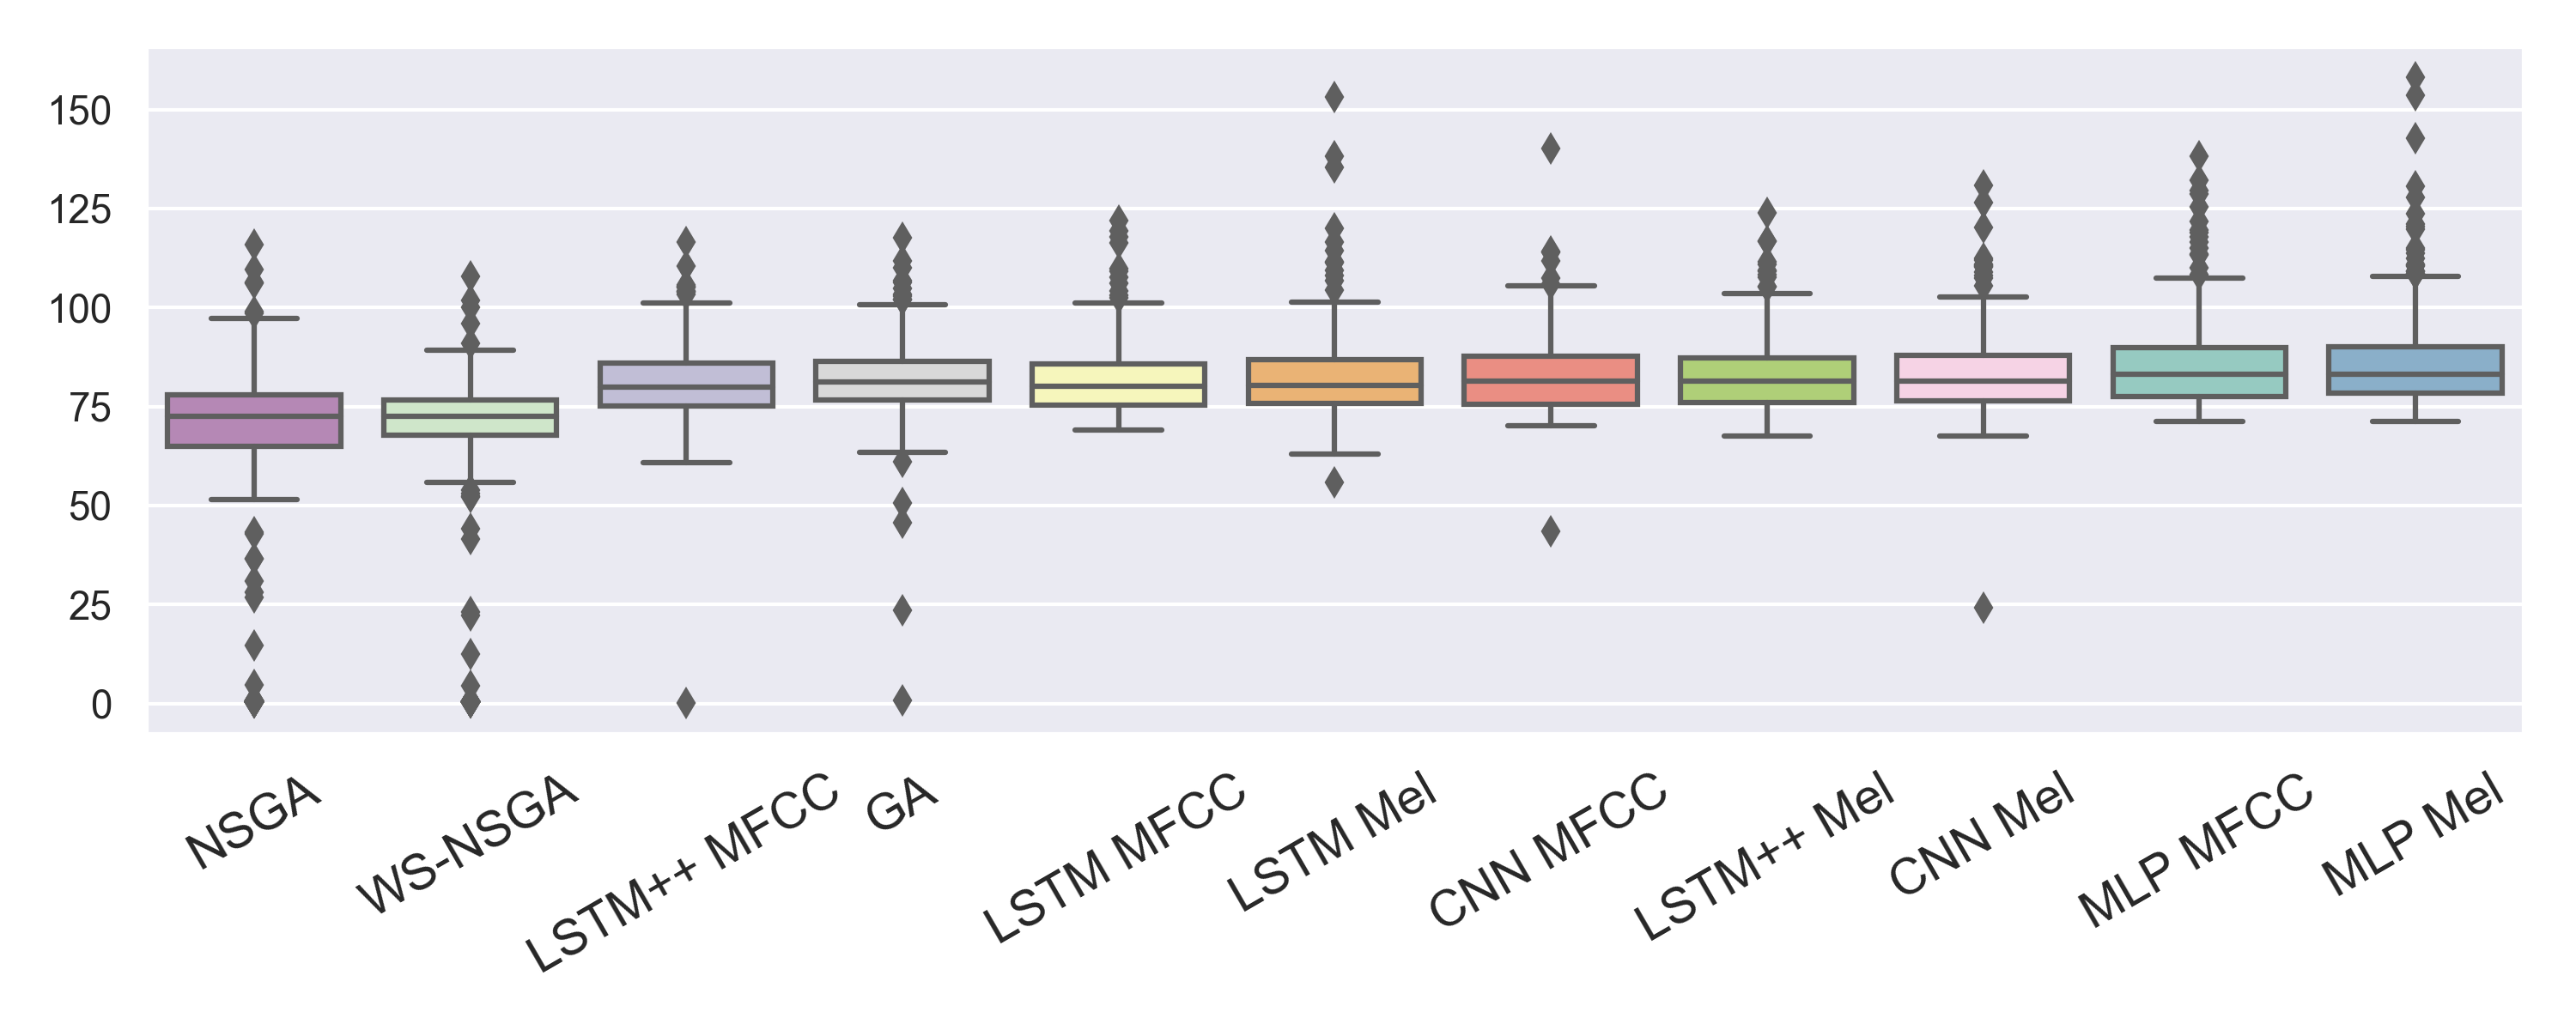
\includegraphics[width=\textwidth]{figures/inverse-synth/lsd_boxplot.png}
        \caption{Log Spectral Distance}
        \label{fig:lsd}
    \end{subfigure}
    \begin{subfigure}[b]{0.99\textwidth}
        \centering
        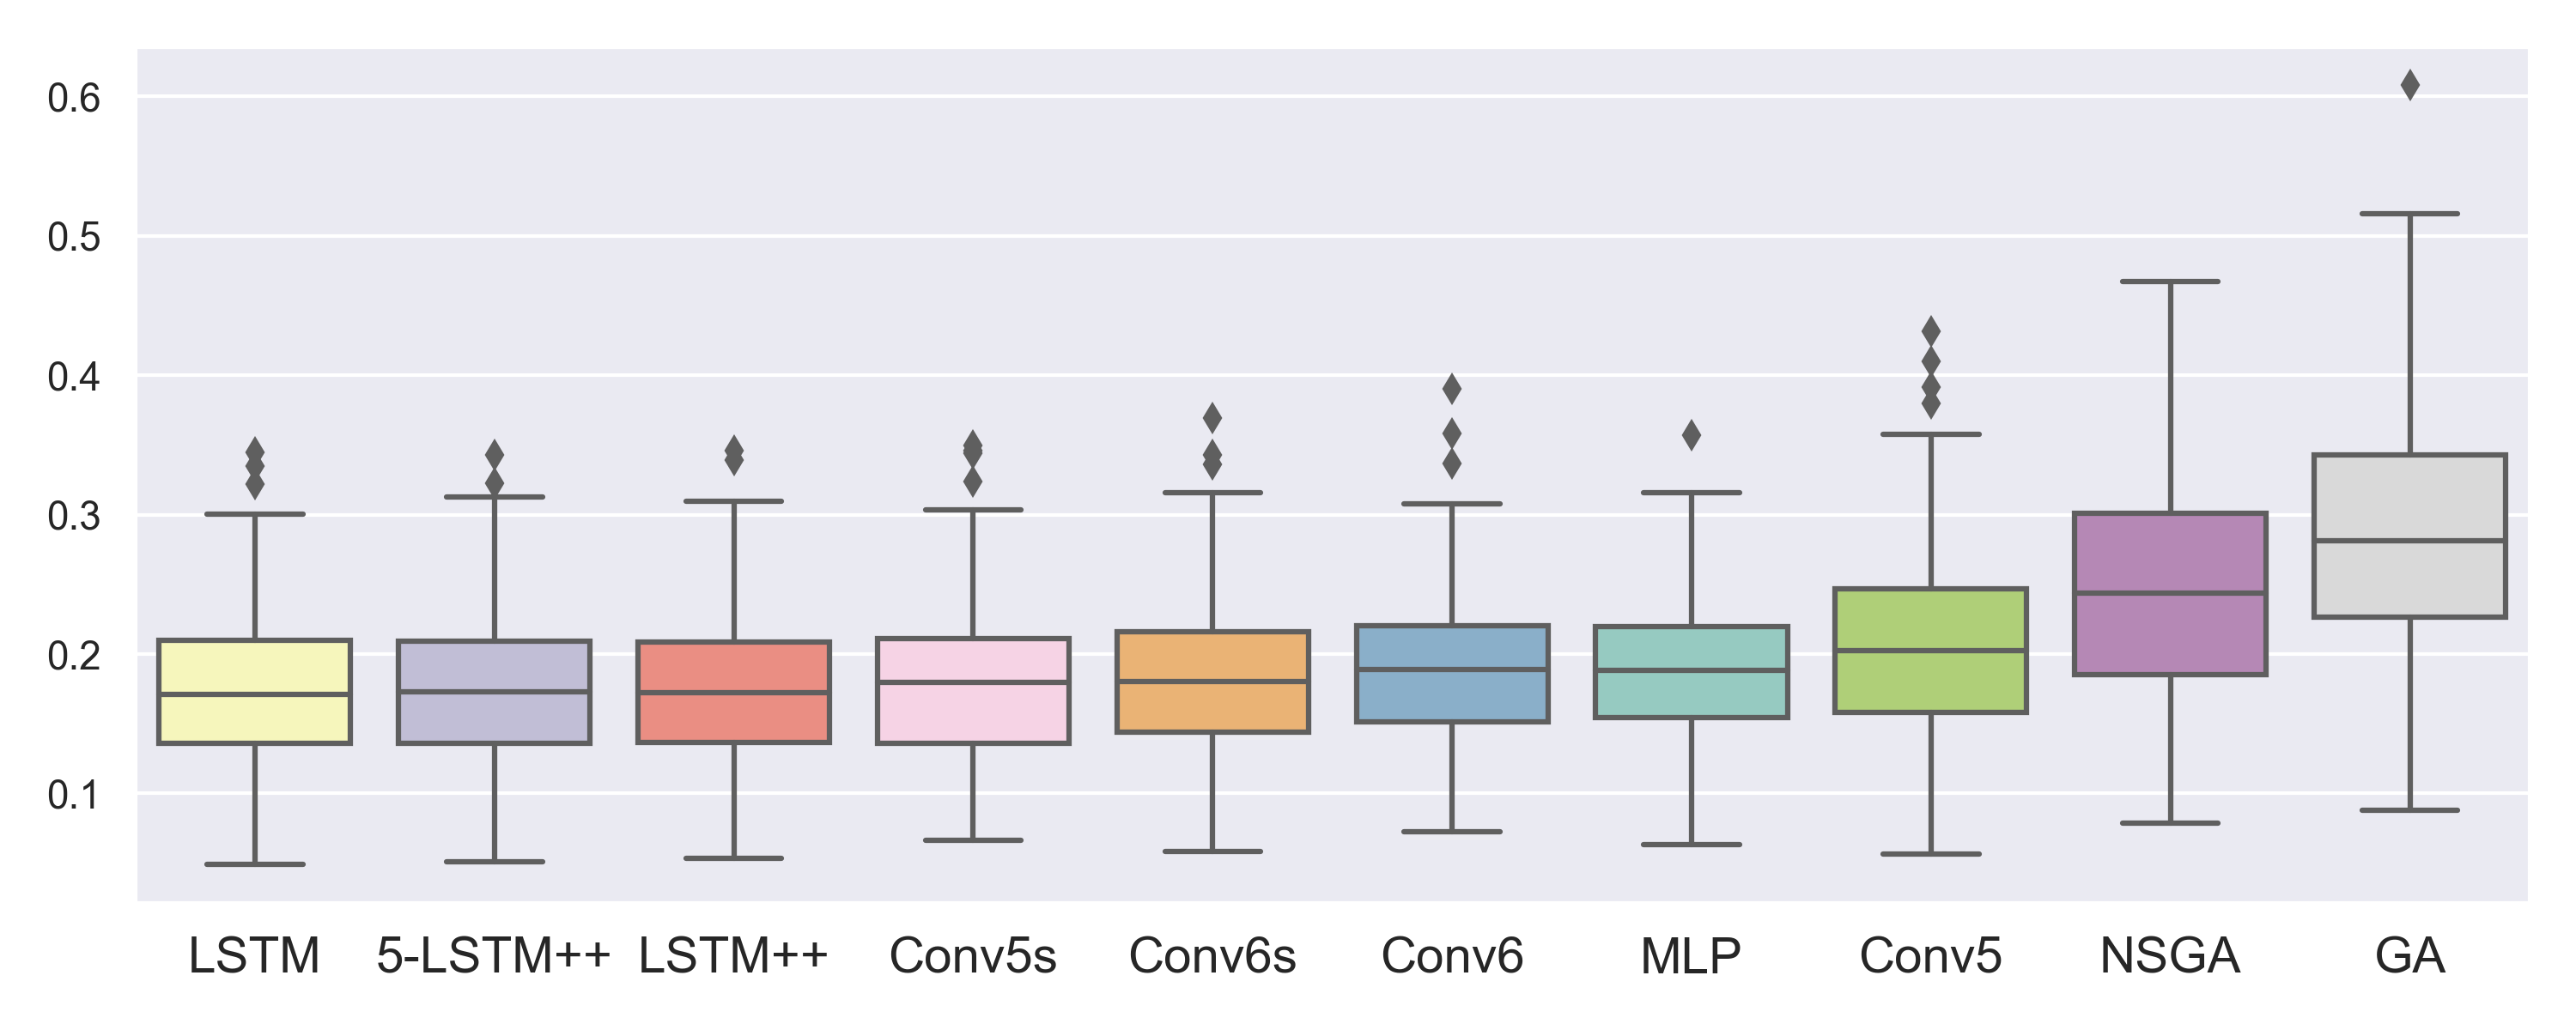
\includegraphics[width=\textwidth]{figures/inverse-synth/parameter_boxplot.png}
        \caption{Parameter MSE}
        \label{fig:param-mse}
    \end{subfigure}
    \caption{Boxplots showing the objective measurements comparing each estimation method using a 250 sample evaluation dataset for sound matching.}
    \label{fig:eval-boxplot}
\end{figure}

\subsection{MFCC Error}
The MFCC error is calculated by computing the mean absolute error between MFCCs from a target audio and a prediction. Yee-King \textit{et al.} \cite{yee2018automatic} also used MFCCs to evaluate the quality of predicted sounds, however they used the euclidian distance between MFCCs as opposed to MAE. The MAE was used here as it showed results in a range that was easier compare. For this evaluation, MFCCs were caclulated using a frame size of 2048 and a hop-size of 512. Figure \ref{fig:mfcc-mae} shows a boxplot graph comparing all the techniques using this metric, ordered by the mean. There is quite high variance for all of the techniques and quite a few outliers with high error, even for the best techniques. However, based on the mean error, the GAs performed the best and the WS-NSGA was overall the best technique. Out of the deep learning models the LSTM models all performed the best, with the two LSTM based methods using MFCCs as input performed the best.

\subsection{Log Spectral Distance}
The log spectral distance (LSD) is a distance metric that is calculated between to power spectrums to quantify difference. It was used by Masuda and Saito as a fitness objective in a genetic algorithm for inverse synthesis \cite{masudo2021quality}. This metric is included to add more depth to the audio evaluation. Masuda and Saito identified a the limitations with calculating error between synthesized sounds using MFCC, particularly with the ability of MFCC to capture specific frequency information as opposed to just the shape of the spectral envelope. LSD provides a more robust evaluation on the spectrograms of the results.  LSD is calculated as:

\begin{equation}
    LSD(P, \hat{P}) = \sqrt{\sum_{\omega}10\text{log}_{10}\left( \frac{P(\omega)}{\hat{P}(\omega)} \right)^2}
\end{equation}

Where $P$ is a target power spectrum, $\hat{P}$ is the power spectrum of a predicted sound, and $\omega$ is a frequency bin. Power spectrums were calculated using a STFT with an FFT size of 1024 samples and a hop-size of 512 samples. The average value of LSD over frames is used as the final evaluation metric in this evaluation. Lower values for LSD indicate a closer match. Figure \ref{fig:lsd} shows a boxplot graph comparing the results of this evaluation. Again, the variance is quite high among all the techniques. Based on the mean LSD the regular NSGA-III approach performed the best, followed closely by the WS-NSGA. The LSTM++ MFCC actually outperformed the basic GA based on this evaluation.

\subsection{Parameter Error}
This metric measures the mean absolute error (MAE) between the parameter values from a target and a prediction. In related work, Barkan \textit{et al.} included this metric to evaluate the distance between target and estimated synthesizer parameters, it is include here for the same reason and to highlight the relationship between the auditory and parameter space. Figure \ref{fig:param-mse} shows a boxplot graph comparing the results of this evaluation. In terms of mean parameter accuracy across testing dataset, all the deep learning models outperformed the NSGA and GA. Interestingly the MFCC-LSTM++ model performed the best out of all the methods, even the WS-NSGA, which used the MFCC-LSTM++ as a starting point. This means that the WS-NSGA in general found parameters that were more different from the target parameters, but resulted in more similar audio matches. These results highlight an important aspect regarding synthesizer programming: poor parameter reconstruction does not necessarily mean poor auditory results.

In addition to calculating the MAE for each target-prediction pair, the absolute error between individual parameters was calculated. This metrics provides insight into how each technique handled the various parameters.

The frequency parameters affect the distribution of the harmonics in the frequency domain, whereas the envelope generator is related to the temporal aspect of the sound and how the frequencies evolve over time. Results for the five parameters related to the envelope generator are shown in table \ref{tbl:param_eval_eg}, and results for the two parameter related to the frequency of operator two are shown in table \ref{tbl:param_eval_osc}.

Results for the EG parameter evaluation show that the WS-NSGA performed the best in determining the rate for first and second stages of the EG, and at determining the level for the third stage. The MFCC-LSTM model was overall the best at estimating parameters for the EG, as well as for the rate of the third stage and the level of the second stage. All methods were most effective at determining the rate of the first stage, followed by the rate and level of the second stage, and worst at the estimating the rate and level of the third stage. The duration of each of the first three stages range from 0 seconds to almost a minute. The length of the note is only one second long, so if the duration of the first stage is one second or longer, then the second and third stages will never be reached and will not be reflected in the audio result. This  means that there are large portions of the synthesizer parameter space that are redundant for a note of one second long.  This redundancy reflects a challenge for automatic synthesizer programming approaches and one of the issues with determining loss based on parameter error.

Looking at the frequency parameters, the MFCC-LSTM++ outperformed all the other methods. This is an interesting result in light of the previously mentioned issues identified with MFCCs and their ability to capture precise frequency values. The Mel-LSTM++, which used Mel-Spectrograms, performed only slightly worse than the MFCC-LSTM++. Overall the LSTM++ models performed the best at determine the frequency tuning and the coarse tuning was estimated more successfully than the fine tuning for all models.


%For the EG, the parameter that each of the methods was able to estimate was the rate of the second stage of the envelope (EG Rate 2). The NSGA III received the lowest parameter error for the EG rate 2 parameter, 0.0097, however scored quite poorly on the remained of the parameters. The parameters of the EG were taken together and averaged for each method, the 5-LSTM++ model performed the best overall on estimating parameters for the EG with an error 0f 0.1328. Turning to the parameters controlling the frequency of the second operator, the coarse tuning parameter was by far the easiest parameter for each of the methods to estimate. Interestingly the MLP model was the best performing approach for both the individual coarse parameter estimation (error of 0.0678) as well when looking at tuning the frequency of the second operator as whole with an error of 0.1881. Looking at the mean across all the results for the parameters for the EG compared to the operator frequency show that overall the techniques were able to correctly select the EG parameters (average error of 0.1577) over the frequency parameters (average error of 0.1958).

% All estimators were run on each one of the 25 target sounds using the \mintinline{python}{SoundMatch} class. This resulted in a set of audio files generated from $Dexed$ using the estimated parameters from each estimator run on each of the 25 target sounds. All of the resulting sounds are available for listening online on the SpiegeLib docs page\footnote{\url{https://spiegelib.github.io/spiegelib/examples/fm_sound_match_pages/fm_sound_match_listen.html}}. Quantitative and qualitative evaluation was conducted on these sounds.

% \subsection{Quantitative Evaluation}
% Evaluation was conducted by comparing the predicted audio files to the target audio using MAE computed on MFCCs, which is the same method that was used during evaluation by Yee-King et al. \cite{yee2018automatic}. Results for mean absolute error (MAE) which have been summarized using mean, standard deviation, minimum, and maximum, are shown for each estimator in table \ref{tbl:sound_match_eval}. Both GAs performed better than the deep learning approaches with the NSGA III having the best overall score. For deep learning approaches, the LSTM++ model achieved the best mean score.

% % TODO informal listening based on MAE so I can comment on the results in terms of MAE

% Histograms of the the MAE were also plotted for each estimator using the \mintinline{python}{plot_hist()} method in \mintinline{python}{EvaluationBase}. Histograms of the MAE for all predictions made by all estimators are shown in figure \ref{fig:group_hist}. These plots clearly show the NSGA III as the winner in terms of MFCC MAE; 24/25 of the predicted sounds have an MAE less than 2.5 (the smallest histogram bin), and the other sound is still less than 5. For the deep learning models, the LSTM++ performed the best overall, however the LSTM model produced more results that had a MAE less than 2.5. The MLP model performed the worst overall and the histogram shows a wide range of results, the MLP also produced a result with the worst individual score of 34.12. The CNN model performed only slightly better than the MLP and had no predictions with a score less than 2.5.

\begin{table}[ht]
\centering
\begin{tabular}{l|ccc|cc|c}
\toprule
{} & \multicolumn{3}{c}{EG Rate} & \multicolumn{2}{c}{EG Level} & {} \\
{} & 1 & 2 & 3 & 2 & 3 & Mean \\
\midrule
MFCC-MLP    &     0.0279 &     0.1048 &     0.2443 &      0.1859 &      0.2072 &   0.1540 \\
MFCC-LSTM   &     0.0129 &     0.0544 &     \textbf{0.2082} &      \textbf{0.1643} &      0.1920 &   \textbf{0.1264} \\
MFCC-LSTM++ &     0.0156 &     0.0533 &     0.2304 &      0.1670 &      0.1929 &   0.1318 \\
MFCC-CNN    &     0.0200 &     0.0621 &     0.2202 &      0.1825 &      0.1911 &   0.1352 \\
\midrule
Mel-MLP     &     0.0379 &     0.1053 &     0.2618 &      0.2036 &      0.1982 &   0.1614 \\
Mel-LSTM    &     0.0190 &     0.0626 &     0.2163 &      0.1811 &      0.1870 &   0.1332 \\
Mel-LSTM++  &     0.0195 &     0.0607 &     0.2241 &      0.1848 &      0.1896 &   0.1357 \\
Mel-CNN     &     0.0203 &     0.0735 &     0.2322 &      0.2023 &      0.1998 &   0.1456 \\
\midrule
GA          &     0.0326 &     0.1786 &     0.3196 &      0.2125 &      0.2812 &   0.2049 \\
NSGA        &     \textbf{0.0095} &     0.0834 &     0.2982 &      0.2464 &      0.2221 &   0.1719 \\
WS-NSGA     &     \textbf{0.0095} &     \textbf{0.0455} &     0.2283 &      0.1712 &      \textbf{0.1850} &   0.1279 \\
\midrule
Mean        &     0.0204 &     0.0804 &     0.2440 &      0.1911 &      0.2042 &   0.1480 \\
\bottomrule
\end{tabular}
\caption{Absolute error on envelope generator parameters, averaged over all test items}
\label{tbl:param_eval_eg}
\end{table}

\begin{table}[ht]
\centering
\begin{tabular}{l|cc|c}
\toprule
{} & \multicolumn{2}{c}{Operator 2 Frequency} & {} \\
{} & Coarse & Fine & Mean \\
\midrule
MFCC-MLP    &    0.0680 &  0.2193 & 0.1437 \\
MFCC-LSTM   &    0.0620 &  0.2061 & 0.1341 \\
MFCC-LSTM++ &    \textbf{0.0599} &  \textbf{0.1817} & \textbf{0.1208} \\
MFCC-CNN    &    0.0661 &  0.1945 & 0.1303 \\
\midrule
Mel-MLP     &    0.0747 &  0.2042 & 0.1394 \\
Mel-LSTM    &    0.0605 &  0.2146 & 0.1376 \\
Mel-LSTM++  &    0.0619 &  0.1835 & 0.1227 \\
Mel-CNN     &    0.0678 &  0.2223 & 0.1451 \\
\midrule
GA          &    0.0971 &  0.2622 & 0.1796 \\
NSGA        &    0.0688 &  0.2196 & 0.1442 \\
WS-NSGA     &    0.0619 &  0.2014 & 0.1317 \\
\midrule
Mean        &    0.0681 &  0.2100 & 0.1390 \\
\bottomrule
\end{tabular}
\caption{Absolute error on operator two frequency parameters, averaged over all test items}
\label{tbl:param_eval_osc}
\end{table}

% Maybe add some spectrograms?
% \subsection{Qualitative Evaluation}
% Spectrograms of one target sound and predictions made by each of the estimators for that target are shown in figure \ref{fig:group_spect}. The selected example was one of the most challenging targets; both the GAs, the LSTM, and the MLP received their worst individual score on it. The most clear difference between the spectrograms can be seen in the temporal evaluation of the harmonics, which is caused by the EG applied to the amplitude of the second operator. In the target the envelope has two obvious components: 1) gradually descending over the first half, and then 2) remaining constant for the remainder of the sound. All the predictions have a similar shape, however only the NSGA III is able to match the shape of of those two sections of the envelope. The MLP, which performed the worst, has two envelope sections, but the first section descends too radpidly and then the constant section is at the incorrect amplitude.

% Another aspect of the spectrograms that can be identified are periodic amplitude modulations occuring along the horizontal axis of the harmonics. These show up as period dark notches on the harmonic. These spacing between the horizontal notches indicates the tuning of the second operator that is modulating the frequency of the first operator. In the target this modulation pattern shows up in the first half of the clip, but not the second. Only the NSGA III was able to correctly match the tuning in both sections of the audio. 

% Did I mess up the charts for the CNN and the GA?? Those shouldn't be different I don't think?

% \begin{figure}[t]
% \begin{center}
% 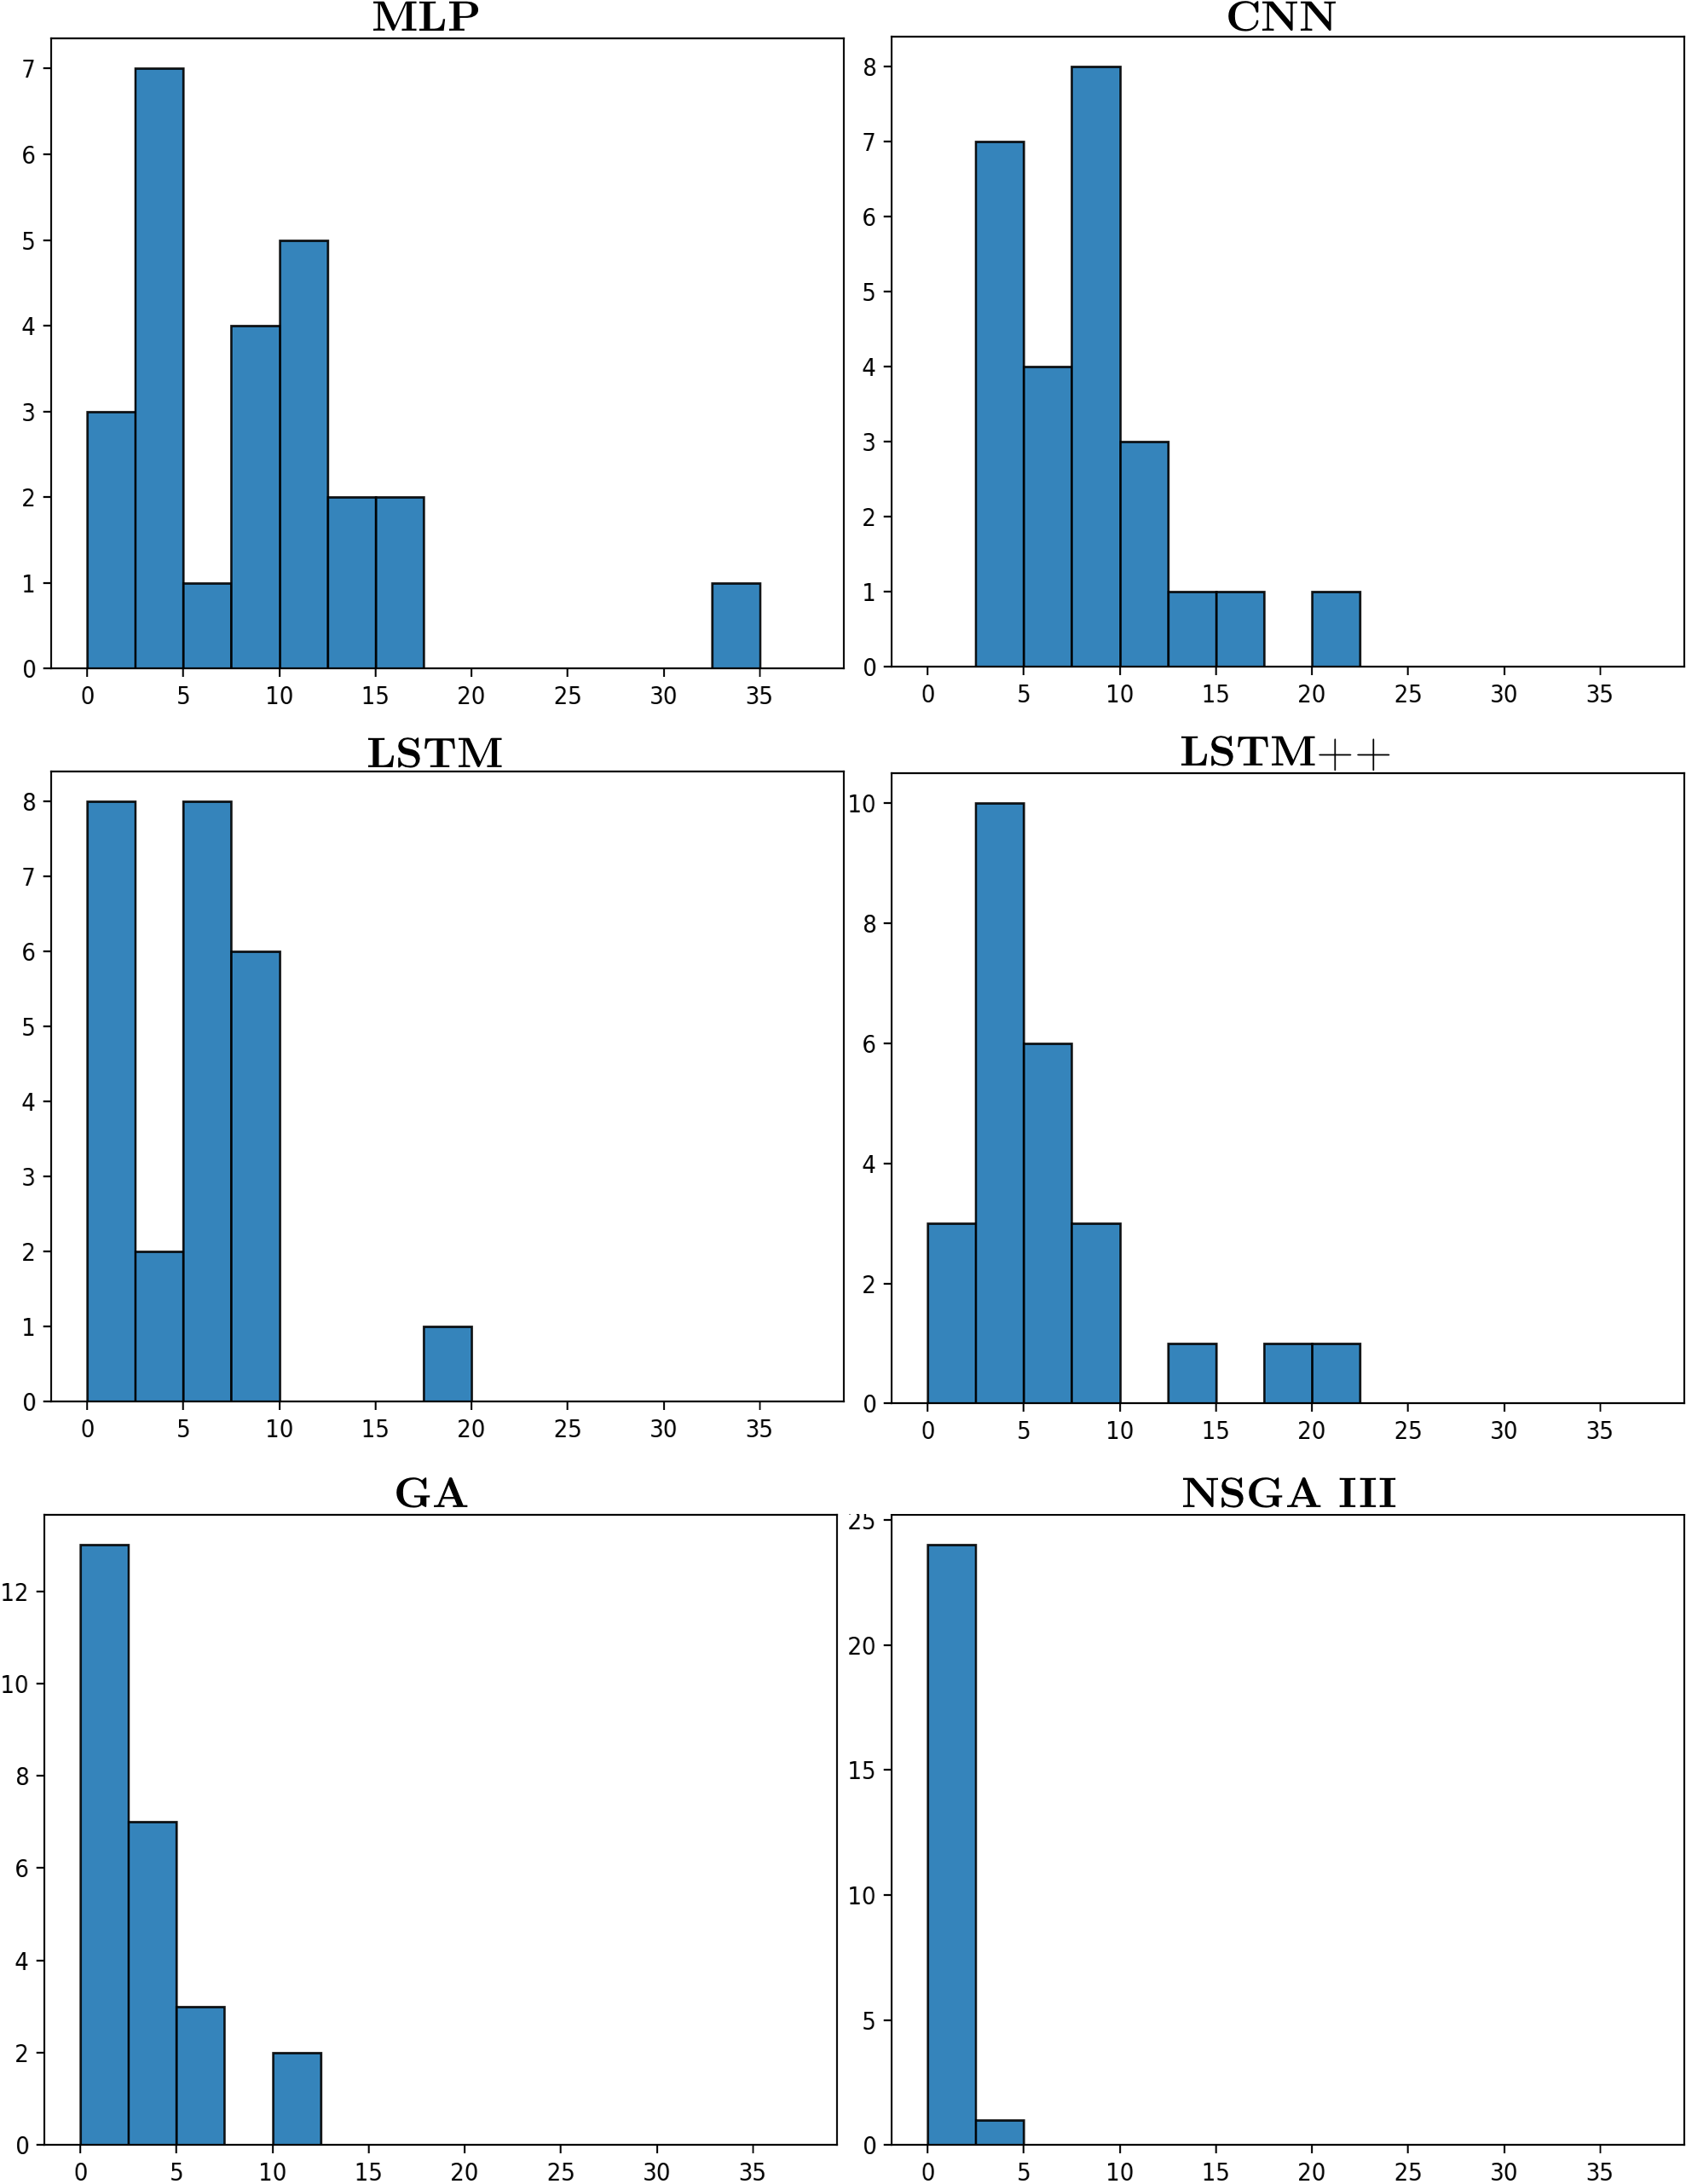
\includegraphics[width=0.75\textwidth]{hist_group_v3.png}
% \caption{Histogram shows the MAE values resulting from MFCC evaluation run on a set of 25 sound targets for all estimators. Lower MAE values indicate a closer sound match.}
% \label{fig:group_hist}
% \end{center}
% \end{figure}

% \begin{figure}[t]
% \begin{center}
% 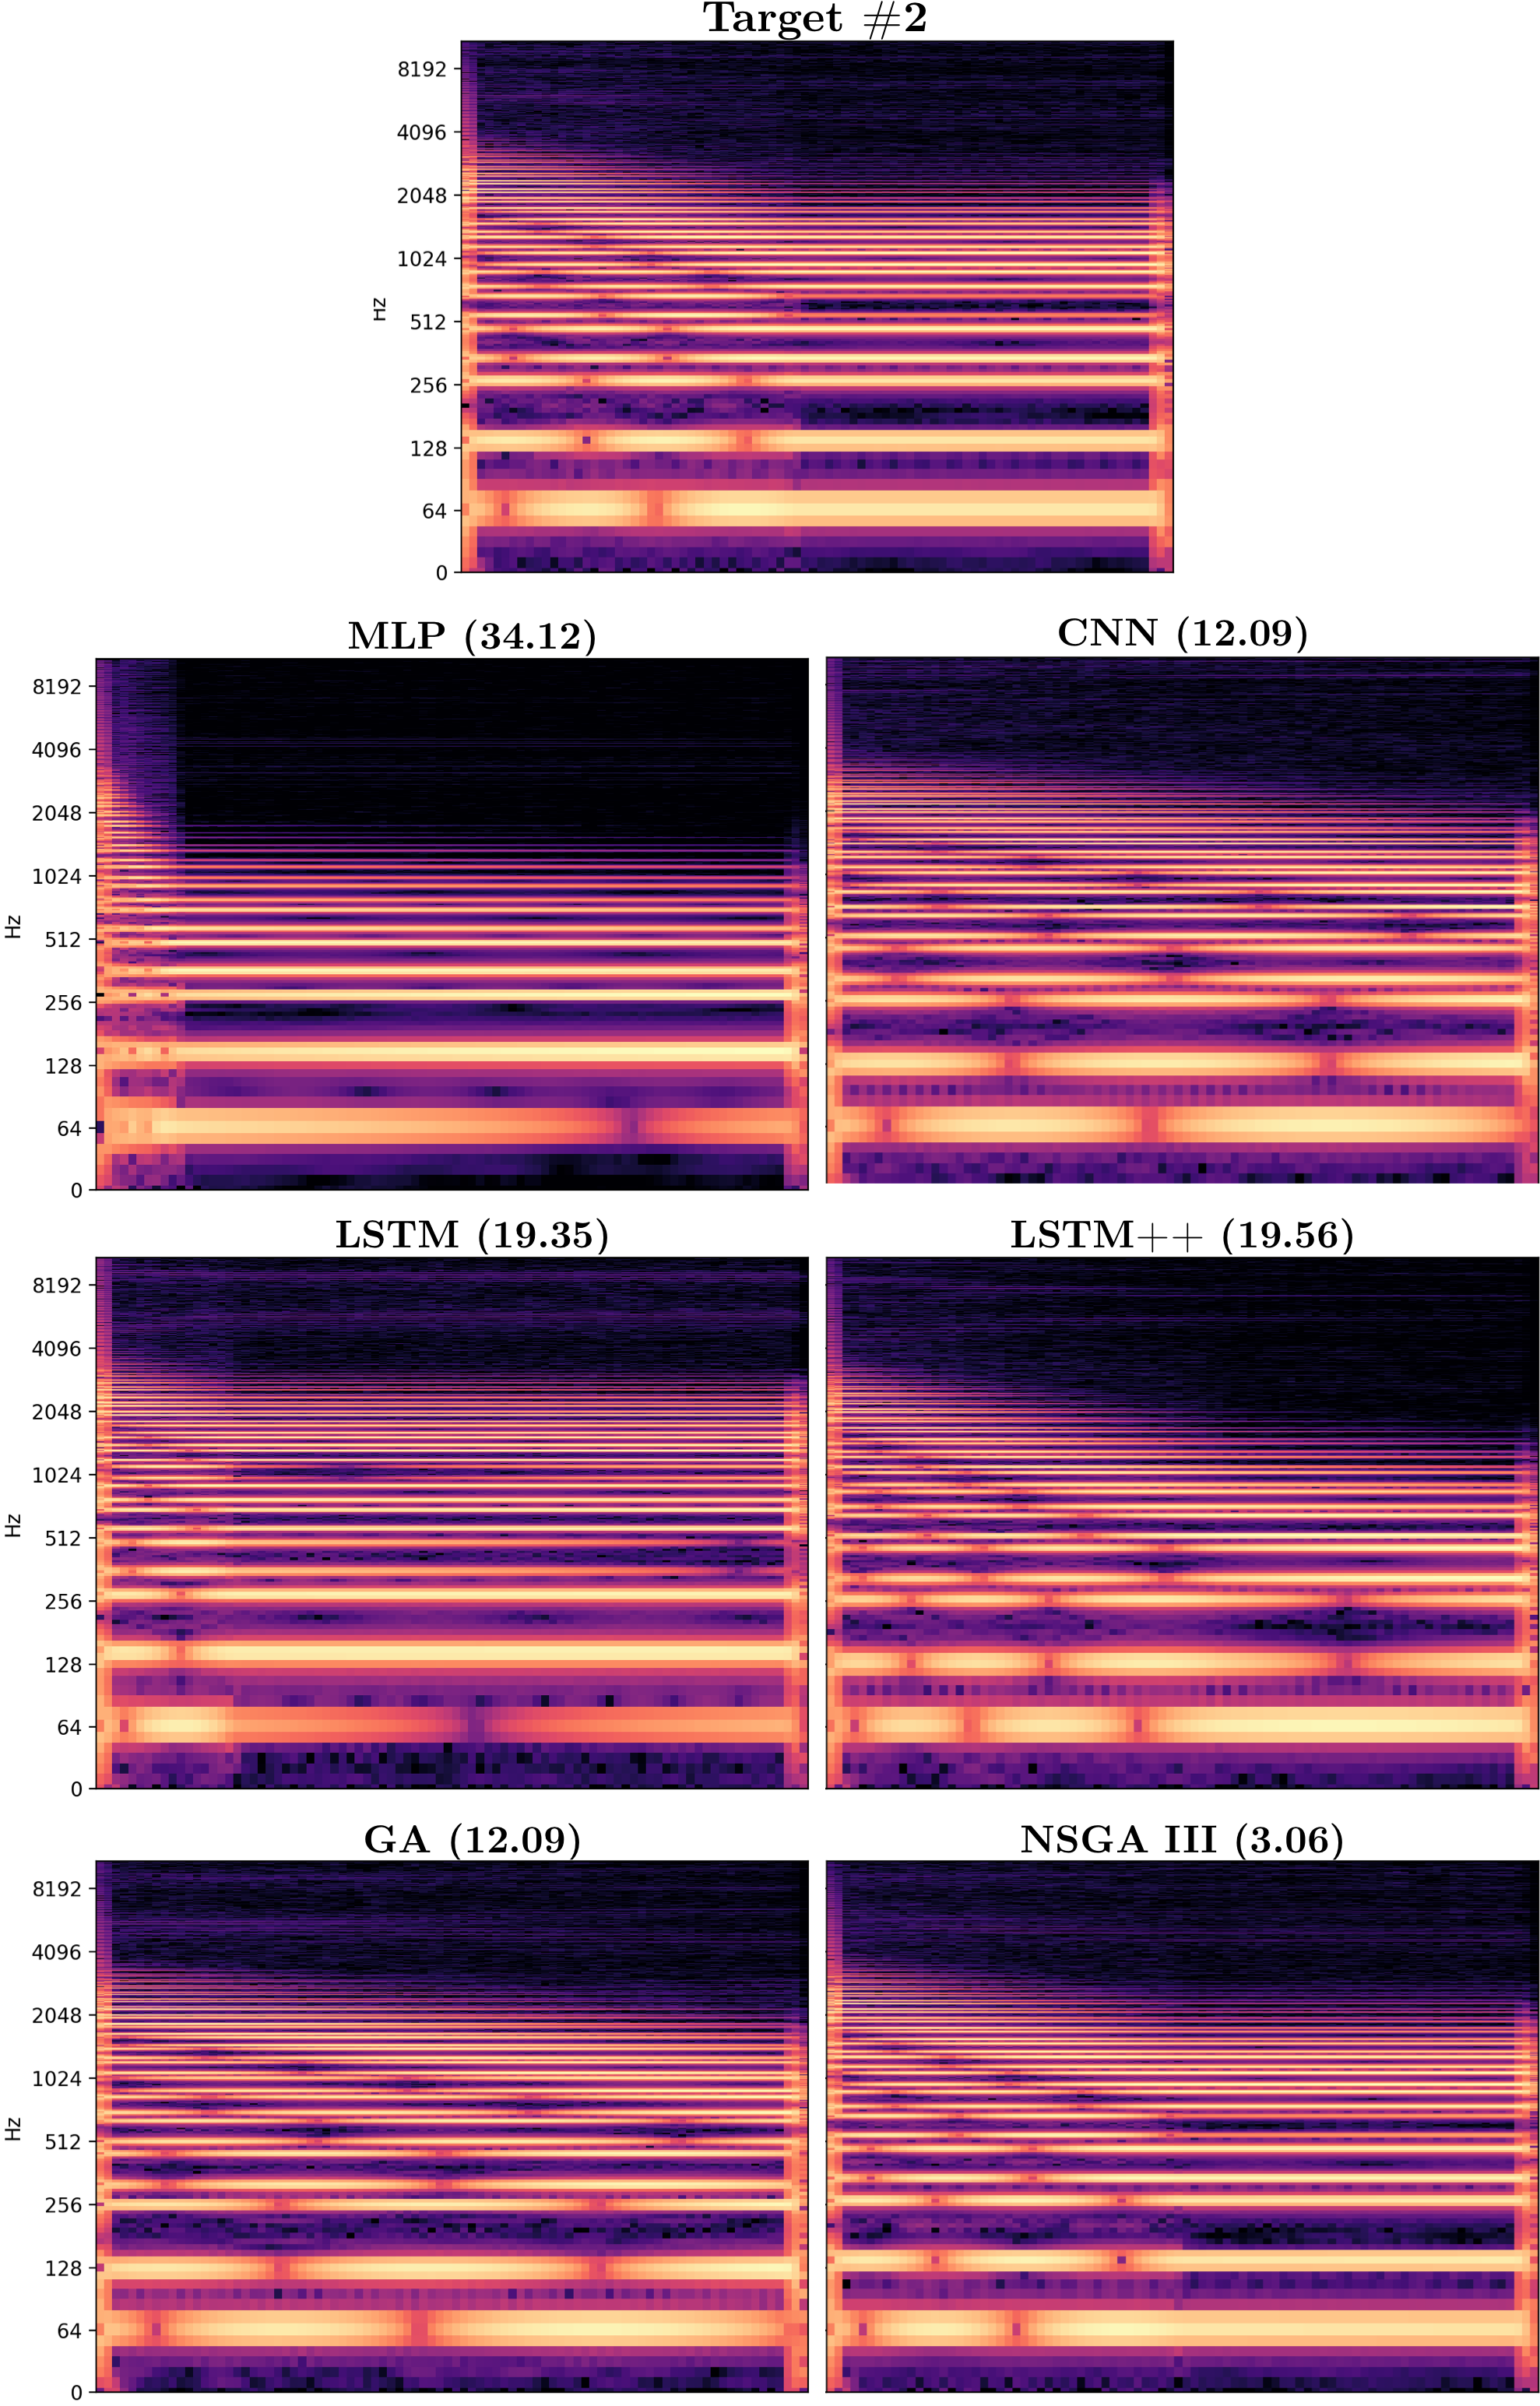
\includegraphics[width=0.75\textwidth]{spect_group_v1.png}
% \caption{Spectrogram plots of a target sound and sound match predictions made by each estimator. The value next to the estimator name is the MAE value from MFCC evaluation for that prediction (lower MAE values indicate a closer match).}
% \label{fig:group_spect}
% \end{center}
% \end{figure}

% I think this can be removed?
% To evaluate to the resulting predictions the \mintinline{python}{MFCCEval} class was used, which calculates error and distance metrics on MFCCs of a target and prediction. Results for mean absolute error (MAE) which have been summarized using mean, standard deviation, minimum, and maximum, are shown for each estimator in table \ref{tbl:sound_match_eval}. Both GAs performed better than the deep learning approaches with the NSGA III having the best overall score. For deep learning approaches, the LSTM++ model achieved the best mean score. Histograms of the the MAE were also plotted for each estimator using the \mintinline{python}{plot_hist()} method in \mintinline{python}{EvaluationBase}. Histograms of the MAE for all predictions made by all estimators are shown in figure \ref{fig:group_hist}. Spectrograms of one target sound and sound match predictions made by each of the estimators for that target are shown in figure \ref{fig:group_spect}. For this particular target, spectrograms reveal that while the frequency and distribution of the harmonics was relatively close for each estimation, all estimators except for the NSGA III struggled with matching the temporal envelope of the spectrum.

\section{Discussion}
\label{sec:inverse-synth-discuss}

\subsection{Deep Learning vs. Genetic Algorithms}
\textbf{RQ1} sought to explore the difference between the deep learning approaches and the genetic algorithms. Results show differences in terms of accuracy as well as computational complexity between the approaches. The regular NSGA-III as well as the WS-NSGA methods outperformed all the other approaches in terms of the audio evaluation metrics. Both these methods were constrained by the number of generations they were allowed to run for in order to reduce the running time; the WS-NSGA was heavily constrained as it was only allowed to run for 10 generations. Despite the constrains both methods produced high quality results. To say with more certainty which approach produces the best results, a formal listening experiment would need to be conducted. However, the fact that the NSGAs were consistently able to produce audio results that more closely resemble the target in terms of both MFCCs and LSD points to the quality of these approaches. 

The GAs had an advantage because they were optimized directly on the audio signal from the specific target, whereas the deep learning models were optimized on the parameter values from a training set. Results from the objective metrics reflected these differences, the deep learning models reproduced the exact parameter values more accurately.

\subsubsection{Time Complexity}
The trade-off between computational complexity and accuracy displayed by the differences in the GAs and deep learning approaches represents one of the main challenges for inverse synthesis. There is motivation for fast inference considering the main application of these methods is in a music production context where the goal is to reduce the time required to program a synthesizer. The results obtained with the WS-NSGA are promising and show how the strengths of each of the GA and deep learning approaches can be combined to mitigate some of their respective weaknesses. Future work is required to evaluate how this approach will scale to programming synthesizers with more parameters.

\subsection{Deep Learning Models}
The second research question in this experiment, \textbf{RQ2}, sought to compare the different types of deep learning models used in this experiment and the types of input that they used. Results show that the RNN based models outperformed the CNN using the same input representation. It is not surprising that the RNN models were more accurately able to model the temporal aspects of the input sound and achieved low error on the parameters associated with the envelope generator. RNNs are specifically designed to model relationships in sequential data, such as the framewise MFCCs. 

An unexpected result was that the LSTM++ model performed the best at estimating the parameters associated with frequency using the MFCC input. This was unexpected based on the comments from Masuda \textit{et al.} regarding the unsuitability of MFCCs for inverse synthesis \cite{masudo2021quality}. One of the issues that was encountered when using the Mel-Spectrogram input as well as the CNN models for both representations is that they were challenging to train. In early experiments many of the models of began overfitting quite early when using the Mel-Spectrograms (see appendix \ref{appendix:training-loss} figures e-h). Even introducing the learning rate schedule and attempting to optimize the learning rate  still lead to difficulties with training and overfitting. Based on the successes that have been realized in other music and audio domains with Mel-Spectrograms and CNNs, I was expecting to achieve better results with these approaches. Investigating alternative training methods and ways of using these approaches for inverse synthesis is an area for future work.

%Results from all the objective metrics showed that the CNNs under-performed the the RNNs in all cases. This was surprising considering the CNNs used as input the Mel-spectrogram, which is higher resolution representation compared to the MFCCs. This was unexpected based on the comments from Masuda \textit{et al.} regarding the unsuitability of MFCCs for inverse synthesis \cite{masudo2021quality}. I was expecting to see that the CNNs would be able to extract more meaningful information from the higher resolution and more perceptually relevant log Mel-spectrograms. Specifically one would expect to see that the relationship between the harmonics and the pitch to be more accurately learned using the Mel-spectrograms. In fact, the MLP model which used MFCCs as input obtained the lowest parameter error for the frequency and detuning parameters.

 

%One of the issues that was encountered with all the convolutional models is that they were challenging to train. In all experiments the models improved quickly initially, and then began to overfit quite quickly as well (see appendix \ref{appendix:training-loss} figures e-h). Even introducing the learning rate schedule resulted in difficulties with training and overfitting. The CNNs consistently started overfitting before the validation loss reached a level comparable to the RNN models.

% Maybe include this
%\subsubsection{Model Capacity}
%Another interesting result is that the CNN with the least capacity, the \textit{Conv5s} model, was able to train with the most stability and achieve the best scores amongst the CNNs. The Conv5s model contained 600k trainable parameters compared to the Conv5 and Conv6 models which each contained over 1M. Even more interestingly is that the best performing model, which was the tuned LSTM, contained only 86k parameters, and only the MLP was smaller. This shows that for contrary to the results from Barkan \textit{et al.} \cite{barkan2019inversynth}, increasing the capacity of the model did not lead to improved results for this task. These results could also be due to inefficiencies in training that are preventing the larger models from training to their full potential. Exploring larger hyperparameter grids during optimization could help with this.

\subsection{Parameters vs. Audio}
The last research question, \textbf{RQ3}, sought to elucidate how the models responded to the different parameters and how that affected the audio results. The difference between the audio metrics and the parameter metrics shows that high error in terms of parameter values does not necessarily mean a high error in terms of the resulting audio. The NSGA method was one of the best methods in terms of auditory error, however, was the second worst method in terms of parameter error. Every deep learning approach outperformed it. The WS-NSGA model was in the top two for all metrics, both auditory and parameter. This further shows that achieving low parameter error is correlated with low auditory error, but is not a necessary condition for it.

%These results point to the fact that there is a many-to-one relationship between parameter settings and synthesized audio. This is an important attribute of the synthesizer parameter space. There is redundancy in the parameter space, and the amount of redundancy depends on the selection of the other parameters. For example, in this specific experiment, if the rate of the second stage of the EG was set to a value equivalent to one second of longer (length of the MIDI note and resulting audio), then that stage of the envelope would be the only one to have any affect on the resulting sound; all values for stages 3 and 4 rate and level would become redundant. This means that a large portion of the parameter space would map to a single audio result. Developing a a deeper understanding of the complexities of the parameter space and how that relates to synthesized audio will be beneficial for future work on synthesizer programming.

% This is one of the benefits of the GAs over the deep learning approaches, the error between the target and the prediction can be measured directly on the audio, as opposed to measuring the error based on the parameter settings. The downside of this is that GAs are mu

\section{Conclusion}
This chapter presented an experiment that compared several different approaches for performing inverse synthesis using an VST emulation of the Yamaha DX7 synthesizer called Dexed. A subset of seven parameters from Dexed was used for this experiment, which turned Dexed from a complex 6-operator FM synthesizer into a relatively simple 2-operator FM synthesizer; this configuration was capable of producing a wide variety of different evolving timbres and provided a benchmark inverse synthesis task for comparing approaches. Eleven different approaches, including eight deep learning models and two genetic algorithm, and a hybrid approach, were evaluated on a test set of sounds. Within the deep learning models, recurrent models were compared to a convolutional model and a baseline fully-connected model. Each of deep learning models were compared using both MFCCs and Mel-Spectrograms for input.

Previous work has shown that genetic algorithms perform best in terms of match accuracy, but suffer from long computation time. Deep learning models are fast during prediction time, but have not been as accurate at inverse synthesis as the genetic algorithms. A hybrid approach was introduced in this chapter that used a pre-trained LSTM++ model during the generation of the initial population for a multi-objective genetic algorithm, a NSGA-III. The resulting method, called warm-start NSGA, or WS-NSGA was able to achieve similar results in terms of auditory accuracy as the NSGA in 40\% of the time. These results show the potential for combining deep learning and genetic algorithms for the inverse synthesis problem.



%\section{Related Work}
%- Go over the three specific papers that SpiegeLib and the experiments are based on.
%- Deep learning: Fully connected and recursive nets: \cite{yee2018automatic}, Convolutional Nets: \cite{barkan2019inversynth}, Genetic Algorithms: \cite{tatar2016automatic}
%
%\subsection{Recurrent Neural Networks}
%One of the first works on the application of deep learning to the inverse synthesis problem was published by Matthew Yee-King et al. \cite{yee2018automatic} in 2018. The main contribution of their work was an experiment that showed the effectiveness of a type of recurrent neural networks (RNN) called long short-term memory (LSTM) networks at sound matching on an FM synthesizer audio plugin. RNNs were developed to handle time-series data and receive ordered data which is successively fed into the network architecture. As data is fed into the networks, activation states are stored internally and help to provide temporal context in latter stages of computation. RNNs have been particularly successful for audio generation problems \cite{oord2016wavenet, engel2017neural}. 
%
%Yee-King er al. also experimented with additional machine learning techniques including genetic algorithm (GA), Hill-climber, and  multi-layer perceptron (MLP) methods. They also compared two RNN models: a regular LSTM network as well as a modified LSTM network that had a bi-directional LSTM layer as well as several highway layers, they called this network an LSTM++. Their methodology compared a set of algorithms on a series of successfully more challenging problems on the open-source FM synthesizer Dexed\footnote{\url{https://asb2m10.github.io/dexed/}}. Each problem was focused on programming a subset of the parameters in Dexed; a larger subset was used for each successive problem. A dataset of audio samples paired with the parameters used to generate the audio was created for training each of the deep learning models. Mel-frequency Cepstral Coefficients (MFCCs) were used as input for each of the models. The results were evaluated by looking at the error between MFCCs from target sound and a predicted sound. Results showed that the hill-climber algorithm and the LSTM++ model performed the best. The LSTM++ model showed significant improvements over the other deep learning methods, however the hill-climber performed the best on a majority of the tasks.
%
%Their methodology and software provided a basis for the work presented in the chapter and in the development of SpiegeLib.
%
%\subsection{Convolutional Neural Networks}
%Barkan et al. explored convolutional neural networks (CNNs) applied to the inverse synthesis problem in their work which presenting InverSynth \cite{barkan2019deep}. The CNN has been used extensively for image related deep learning tasks and has recently been used successfully in music and audio related tasks including music genre classification \cite{choi2016automatic} and neural audio generation \cite{donahue2018adversarial}. A key feature of CNNs is the use of shared filters that perform convolutions and produce representations at various levels of specificity. The shared filters has allowed them to process large input data such as images and audio with relatively few parameters compared to their fully connected counterparts. 
%
%In their work, Barkan et al. experiment with several different CNN architectures and compare them to a few different fully-connected networks. The focus of their research is performing inverse synthesis on a custom built four oscillator FM synthesizer. They frame the inverse synthesis problem as a classification problem and quantize each of the 23 continuous synthesizer parameters into 16 discrete states. As input they experiment with both STFT as well as raw time-domain audio. Because of the size of these input they created different input representations for the fully-connected networks, for these they used a selection of hand-picked audio features defined in work by Itoyama et al. \cite{itoyama2014parameter}.
%
%Results were evaluated using four different objective methods which evaluate both the ability of the model to match the parameters as well as to reconstruct the target audio. The evaluation metrics used are:
%1) Mean Percentile Rank (MPR): ranked position of the correct class measured against predicted classes in the output. Computed independently on each of the 23 synthesizer parameters, each parameter has 16 classes.
%2) Top-k Mean Accuracy: measures whether the correct class is among the top-k predicted classes for each parameter.
%3) Mean Absolute Error (MAE): this measures the error of the predicted class for each parameter.
%4) Spectral Reconstruction Quality: predicted parameters are used to synthesize a predicted audio. The predicted audio is compared against the target audio using error metrics calculated on the STFT and FT representations.
%
%They also conducted a subjective listening experiment which measured the quality of the target audio to the predicted audio for a selection of the methods. Results from the objective and subjective evaluation showed that the depth of the convolutional network played an important role in the quality of the estimator and the best performing networks were two different networks with 6-layers.


% \begin{table}[t]
% \centering
% \caption{Results from sound matching evaluation}
% \label{tbl:sound_match_eval}
% \begin{threeparttable}
% \begin{tabular}{l|cccc}
% \toprule
% $Method$ & $Mean$ & $SD$ & $Min$ & $Max$ \\
% \midrule
% $MLP$ & 8.55 & 6.77 & 1.92 & 34.12 \\
% $CNN$ & 7.88 & 4.26 & 2.68 & 20.89 \\
% $LSTM$ & 6.12 & 3.76 & 1.20 & 19.36 \\
% $LSTM++$ & 4.91 & 6.50 & 2.12 & 21.51 \\
% $GA$ & 2.25 & 2.58 & 0.70 & 11.17 \\
% $NSGA III$ & \textbf{0.81} & \textbf{0.89} & \textbf{0.001} & \textbf{3.06} \\
% \bottomrule
% \end{tabular}
% \begin{tablenotes}[para, flushleft]
% \footnotesize
% \item Values shown are calculated from the mean absolute error (MAE) calculated during MFCC evaluation. Smaller MAE values indicate more similar matches. The NSGA III estimator received the best scores, which are shown in bold font.
% \end{tablenotes}
% \end{threeparttable}
% %\vspace{5mm}
% \end{table}